% Choose one to switch betweeen slides and handout
%\documentclass[]{beamer}
\documentclass[handout]{beamer}

% Video Meta Data
\title{Bitcoin, Blockchain and Cryptoassets}
\subtitle{Bitcoin Primer}
\author{Prof. Dr. Fabian Schär}
\institute{University of Basel}

% Config File
% Packages
\usepackage[utf8]{inputenc}
\usepackage{hyperref}
\usepackage{gitinfo2}
\usepackage{tikz}
\usepackage{amsmath}
\usepackage{bibentry}
\usepackage{xcolor}
\usepackage{colortbl} % Add colour to LaTeX tables
\usepackage{caption}
\usepackage[export]{adjustbox}
\usepackage{pgfplots} \pgfplotsset{compat = 1.17}

% Color Options
\definecolor{highlight}{rgb}{0.65,0.84,0.82}
\definecolor{focus}{rgb}{0.72, 0, 0}

% Beamer Template Options
\beamertemplatenavigationsymbolsempty
\setbeamertemplate{footline}[frame number]
\setbeamercolor{structure}{fg=black}
\setbeamercolor{footline}{fg=black}
\setbeamercolor{title}{fg=black}
\setbeamercolor{frametitle}{fg=black}
\setbeamercolor{item}{fg=black}
\setbeamercolor{}{fg=black}
\setbeamercolor{bibliography item}{fg=black}
\setbeamercolor*{bibliography entry title}{fg=black}
\setbeamertemplate{items}[square]
\setbeamertemplate{enumerate items}[default]
\captionsetup[figure]{labelfont={color=black},font={color=black}}
\captionsetup[table]{labelfont={color=black},font={color=black}}

\setbeamertemplate{bibliography item}{\insertbiblabel}

% Link Icon Command
\newcommand{\link}{%
    \tikz[x=1.2ex, y=1.2ex, baseline=-0.05ex]{%
        \begin{scope}[x=1ex, y=1ex]
            \clip (-0.1,-0.1)
                --++ (-0, 1.2)
                --++ (0.6, 0)
                --++ (0, -0.6)
                --++ (0.6, 0)
                --++ (0, -1);
            \path[draw,
                line width = 0.5,
                rounded corners=0.5]
                (0,0) rectangle (1,1);
        \end{scope}
        \path[draw, line width = 0.5] (0.5, 0.5)
            -- (1, 1);
        \path[draw, line width = 0.5] (0.6, 1)
            -- (1, 1) -- (1, 0.6);
        }
    }

% Read Git Data from Github Actions Workflow
% Defaults to gitinfo2 for local builds
\IfFileExists{gitInfo.txt}
	{\input{gitInfo.txt}}
	{
		\newcommand{\gitRelease}{(Local Release)}
		\newcommand{\gitSHA}{\gitHash}
		\newcommand{\gitDate}{\gitAuthorIsoDate}
	}

% Custom Titlepage
\defbeamertemplate*{title page}{customized}[1][]
{
  \vspace{-0cm}\hfill
\includegraphics[width=2.5cm]{../config/logo_cif}
  
\includegraphics[width=1.9cm]{../config/seal_wwz}
  \\ \vspace{2em}
  \usebeamerfont{title}\textbf{\inserttitle}\par
  \usebeamerfont{title}\usebeamercolor[fg]{title}\insertsubtitle\par  \vspace{1.5em}
  \small\usebeamerfont{author}\insertauthor\par
  \usebeamerfont{author}\insertinstitute\par \vspace{2em}
  \usebeamercolor[fg]{titlegraphic}\inserttitlegraphic
    \tiny \noindent \texttt{Release Ver.: \gitRelease}\\ 
    \texttt{Version Hash: \gitSHA}\\
    \texttt{Version Date: \gitDate}\\ \vspace{1em}
  \link \href{https://github.com/cifunibas/Bitcoin-Blockchain-Cryptoassets/blob/main/slides/intro.pdf}
  {Get most recent version}\\
  \link \href{https://github.com/cifunibas/Bitcoin-Blockchain-Cryptoassets/blob/main/slides/intro.pdf}
  {Watch video lecture}\\ \vspace{1em}
  License: \texttt{Creative Commons Attribution-NonCommercial-ShareAlike 4.0 International}\\\vspace{2em}
  
\includegraphics[width = 1.2cm]{../config/license}
}

% tikzlibraries
\usetikzlibrary{decorations.pathreplacing}
\usetikzlibrary{decorations.markings}
\usetikzlibrary{positioning}

%caption font
\captionsetup{font=footnotesize}

%%%%%%%%%%%%%%%%%%%%%%%%%%%%%%%%%%%%%%%%%%%%%%
%%%%%%%%%%%%%%%%%%%%%%%%%%%%%%%%%%%%%%%%%%%%%%
\begin{document}

\thispagestyle{empty}
\begin{frame}[noframenumbering]
	\titlepage
\end{frame}

%%%
\begin{frame}{Let's Begin}
	\center
	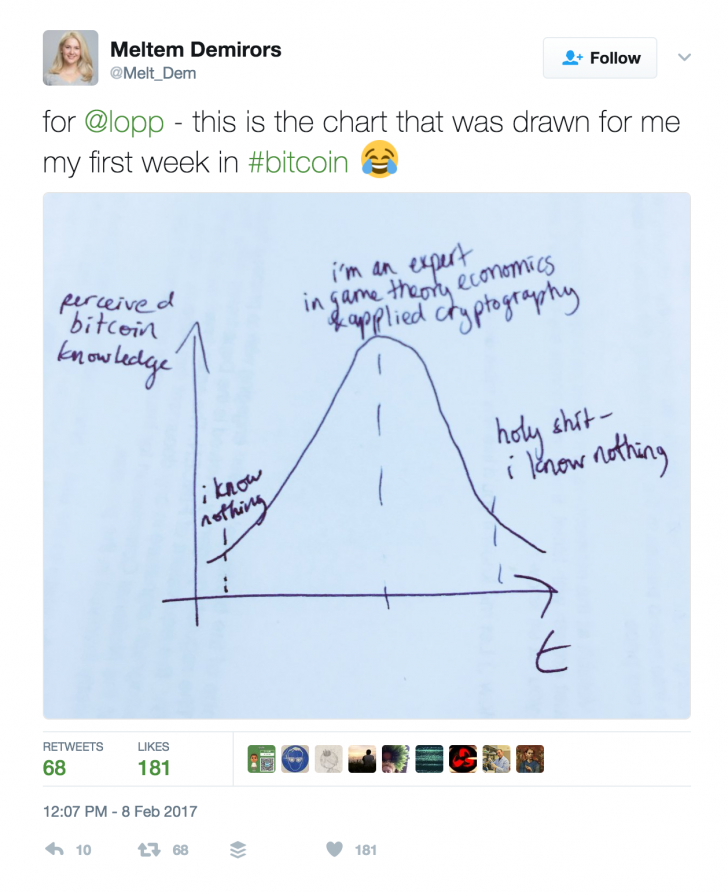
\includegraphics[width=6cm]{../assets/images/meltem_tweet}
\end{frame}
%%%

%%%
\begin{frame}{What We Already Know...}
\textbf{Bitcoin key characteristics:}
	\begin{enumerate}
		\item Competitive creation
		\item Virtual representation
		\item Decentralized management
		\begin{itemize}
			\item Transaction capacity
			\item Transaction legitimacy
			\item Transaction consensus
		\end{itemize}
	\end{enumerate}
	\vspace{1em}
	\uncover<2->{
	\textbf{Key Idea:}\\
	\uncover<2->{Bitcoin is a decentralized data structure.}
	\uncover<2->{The system is maintained by its participants and works in the absence of centralized third parties.}
	}
\end{frame}
%%%

%%%
\begin{frame}{Bitcoin Building Blocks}
	\begin{figure}[h!]
		\center
		%%
\begin{figure}[h!]
  \center
  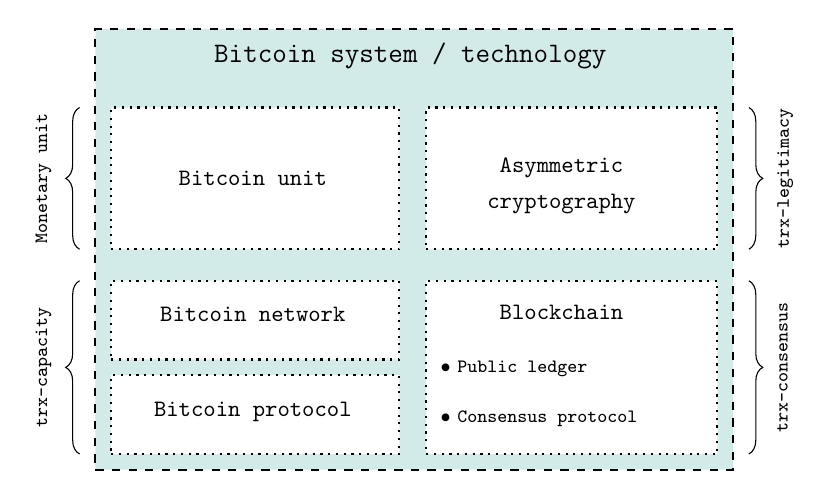
\begin{tikzpicture}[domain=0:10,scale=0.8, every node/.style={scale=0.85}]
    \draw[dashed, thick, fill=highlight!50] (0,0) -- (10.125,0) -- (10.125,7) -- (0,7) -- (0,0);
    

    \draw[dotted, thick,fill=white] (0.25,0.25) -- (4.825,0.25) -- (4.825,1.5) -- (0.25,1.5) -- (0.25,0.25);  
    \draw[color=black] (2.5,0.925) node{\texttt{Bitcoin protocol}};
    
    \draw[dotted, thick,fill=white] (0.25,1.75) -- (4.825,1.75) -- (4.825,3) -- (0.25,3) -- (0.25,1.75);
    \draw[color=black] (2.5,2.475) node{\texttt{Bitcoin network}};  
        
    \draw[dotted, thick,fill=white] (0.25,3.5) -- (4.825,3.5) -- (4.825,5.75) -- (0.25,5.75) -- (0.25,3.5);
    \draw[color=black] (2.5,4.625) node{\texttt{Bitcoin unit}};    
    
    \draw[dotted, thick,fill=white] (5.25,0.25) -- (9.875,0.25) -- (9.875,3) -- (5.25,3) -- (5.25,0.25);
    \draw[color=black] (7.4,2.25) node[above]{\texttt{Blockchain}};   
    \draw[color=black] (5.35,1.6) node[right]{\footnotesize{$\bullet$ \texttt{Public ledger}}};   
    \draw[color=black] (5.35,0.8) node[right]{\footnotesize{$\bullet$ \texttt{Consensus protocol}}};
    
    \draw[dotted, thick,fill=white] (5.25,3.5) -- (9.875,3.5) -- (9.875,5.75) -- (5.25,5.75) -- (5.25,3.5);
    \draw[color=black] (7.4,4.5) node[above]{\texttt{Asymmetric}} node[below]{\texttt{cryptography}};      

    \draw (5,6.9)node[below]{\large{\texttt{Bitcoin system / technology}}};
    
    \draw [decorate,decoration={brace,amplitude=5pt},xshift=0pt,yshift=0pt]
  	(-0.25,0.25) -- (-0.25,3) node [above,black,midway,xshift=-0.3cm,rotate=90]{\footnotesize \texttt{trx-capacity}};

    \draw [decorate,decoration={brace,amplitude=5pt,mirror},xshift=0pt,yshift=0pt]
 	(10.375,0.25) -- (10.375,3) node [below,black,midway,xshift=0.3cm,rotate=90] 
 	{\footnotesize \texttt{trx-consensus}};

    \draw [decorate,decoration={brace,amplitude=5pt},xshift=0pt,yshift=0pt]
	(-0.25,3.5) -- (-0.25,5.75) node [above,black,midway,xshift=-0.3cm,rotate=90] 
	{\footnotesize \texttt{Monetary unit}};

   	\draw [decorate,decoration={brace,amplitude=5pt,mirror},xshift=0pt,yshift=0pt]
	(10.375,3.5) -- (10.375,5.75) node [below,black,midway,xshift=0.3cm,rotate=90] 
	{\footnotesize \texttt{trx-legitimacy}};
    
  \end{tikzpicture}
  %\caption{Overview Bitcoin-system (trx = transaction)}
  \label{fig:bitcoinsystem}
\end{figure}
%%
		\label{fig:bitcoinsystem}
	\end{figure}
\end{frame}
%%%

%%%
\begin{frame}{Transaction Capacity}
\textbf{Goal:} Ensure that each participant can reliably \color{focus}initiate a transaction \color{black} without having to fear censorship. \\
\uncover<2->{
	\begin{figure}[h!]
		\center
		\begin{figure}[h!]
\center
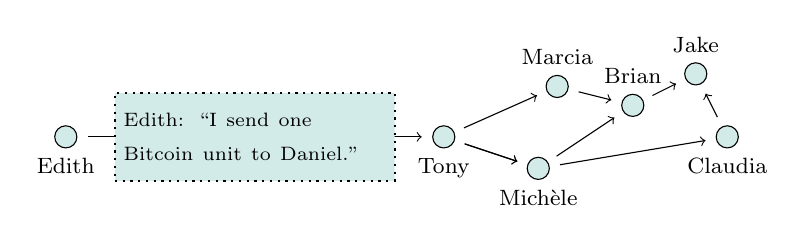
\begin{tikzpicture}[domain=-8:8, scale=0.8]
\coordinate (c1) at (0,0);
\coordinate (c2) at (6,0);
\coordinate (c3) at (7.8,0.8);
\coordinate (c4) at (7.5,-0.5);
\coordinate (c5) at (9,0.5);
\coordinate (c6) at (10,1);
\coordinate (c7) at (10.5,0);
\filldraw[draw=black,fill=highlight!50] (c1) circle (5pt) node[below=0.15cm,color=black]{\footnotesize{Edith}};
\filldraw[draw=black,fill=highlight!50] (c2) circle (5pt) node[below=0.15cm,color=black]{\footnotesize{Tony}};
\filldraw[draw=black,fill=highlight!50] (c3) circle (5pt) node[above=0.15cm,color=black]{\footnotesize{Marcia}};
\filldraw[draw=black,fill=highlight!50] (c4) circle (5pt) node[below=0.15cm,color=black]{\footnotesize{Michèle}};
\filldraw[draw=black,fill=highlight!50] (c5) circle (5pt) node[above=0.15cm,color=black]{\footnotesize{Brian}};
\filldraw[draw=black,fill=highlight!50] (c6) circle (5pt) node[above=0.15cm,color=black]{\footnotesize{Jake}};
\filldraw[draw=black,fill=highlight!50] (c7) circle (5pt) node[below=0.15cm,color=black]{\footnotesize{Claudia}};

\draw[shorten >=0.28cm,shorten <=0.28cm,->] (c1) to[] (c2);
\draw[shorten >=0.28cm,shorten <=0.28cm,->] (c2) to[] (c3);
\draw[shorten >=0.28cm,shorten <=0.28cm,->] (c2) to[] (c4);
\draw[shorten >=0.28cm,shorten <=0.28cm,->] (c2) to[] (c4);
\draw[shorten >=0.28cm,shorten <=0.28cm,->] (c3) to[] (c5);
\draw[shorten >=0.28cm,shorten <=0.28cm,->] (c4) to[] (c5);
\draw[shorten >=0.28cm,shorten <=0.28cm,->] (c4) to[] (c7);
\draw[shorten >=0.28cm,shorten <=0.28cm,->] (c5) to[] (c6);
\draw[shorten >=0.28cm,shorten <=0.28cm,->] (c7) to[] (c6);

\filldraw[fill=highlight!50,dotted,thick] (0.78,-0.7) -- (5.22,-0.7) -- (5.22,0.7) -- (0.78,0.7) -- (0.78,-0.7) node[midway, right=-0.02cm,text width=4.25cm]{\scriptsize{Edith: ``I send one \\ Bitcoin unit to Daniel.''}};

\end{tikzpicture}
\end{figure}\vspace{1em}

	\end{figure}\vspace{1em}
}
\uncover<2->{
	Peer-to-Peer Network:
        \begin{itemize}
		\item<1-> Permissionless
		\item<1-> Censorship-resistant
		\item<1-> No special privileges
		\end{itemize}
		}
\end{frame}
%%%


%%%
\begin{frame}{Transaction Legitimacy}
\textbf{Goal:} Ensure transaction \color{focus}authenticity \color{black}and \color{focus} integrity\color{black}, i.e., ensure that the transaction was initiated by its owner of the funds and has not been changed.
\uncover<2->{
		\center
		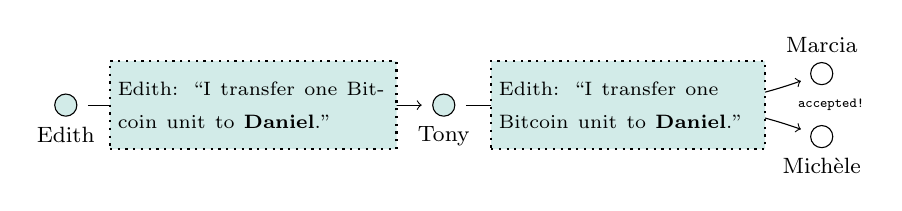
\begin{tikzpicture}[domain=-8:8, scale=0.8]
\coordinate (c1) at (0,0);
\coordinate (c2) at (6,0);
%\coordinate (c3) at (7.8,0.8);
%\coordinate (c4) at (7.5,-0.5);
%\coordinate (c5) at (9,0.5);
%\coordinate (c6) at (10,1);
%\coordinate (c7) at (10.5,0);
\filldraw[draw=black,fill=highlight!50] (c1) circle (5pt) node[below=0.15cm,color=black]{\footnotesize{Edith}};
\filldraw[draw=black,fill=highlight!50] (c2) circle (5pt) node[below=0.15cm,color=black]{\footnotesize{Tony}};

\draw[shorten >=0.28cm,shorten <=0.28cm,->] (c1) to[] (c2);
\draw[shorten >=0.28cm,shorten <=0.28cm,->] (c2) to[] (9,0);
\draw[shorten >=0.28cm,shorten <=0.28cm,->] (9,0) to[bend right = 10] (12,0.5);
\draw[shorten >=0.28cm,shorten <=0.28cm,->] (9,0) to[bend left = 10] (12,-0.5);

\filldraw[draw=black,fill=white] (12,0.5) circle (5pt) node[above=0.15cm,color=black]{\footnotesize{Marcia}};
\filldraw[draw=black,fill=white] (12,-0.5) circle (5pt) node[below=0.15cm,color=black]{\footnotesize{Michèle}};


\filldraw[fill=highlight!50,dotted,thick] (0.7,-0.7) -- (5.25,-0.7) -- (5.25,0.7) -- (0.7,0.7) -- (0.7,-0.7) node[midway, right=-0.03cm,text width=3.5cm]{\scriptsize{Edith: ``I transfer one Bitcoin unit to \textbf{Daniel}.''}};

\filldraw[fill=highlight!50,dotted,thick] (6.75,-0.7) -- (11.1,-0.7) -- (11.1,0.7) -- (6.75,0.7) -- (6.75,-0.7) node[midway, right=-0.03cm,text width=3.3cm]{\scriptsize{Edith: ``I transfer one Bitcoin unit to \textbf{Daniel}.''}};

\draw (12.15,0) node[color=black]{\tiny{\texttt{accepted!}}};

\end{tikzpicture}

		}
\uncover<3->{
		\vspace{2em}
		\begin{figure}[h!]
\center
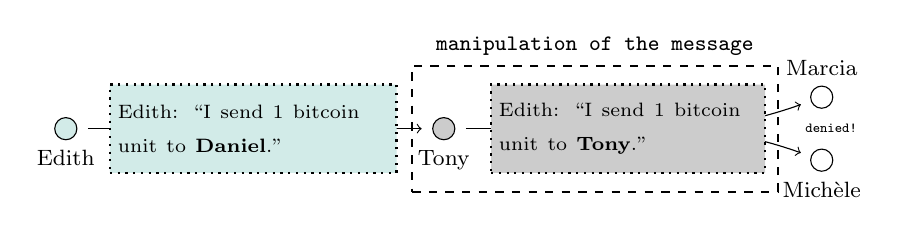
\begin{tikzpicture}[domain=-8:8, scale=0.8]
\coordinate (c1) at (0,0);
\coordinate (c2) at (6,0);
%\coordinate (c3) at (7.8,0.8);
%\coordinate (c4) at (7.5,-0.5);
%\coordinate (c5) at (9,0.5);
%\coordinate (c6) at (10,1);
%\coordinate (c7) at (10.5,0);
\filldraw[draw=black,fill=highlight!50] (c1) circle (5pt) node[below=0.15cm,color=black]{\footnotesize{Edith}};
\filldraw[draw=black,fill=black!20] (c2) circle (5pt) node[below=0.15cm,color=black]{\footnotesize{Tony}};

\draw[shorten >=0.28cm,shorten <=0.28cm,->] (c1) to[] (c2);
\draw[shorten >=0.28cm,shorten <=0.28cm,->] (c2) to[] (9,0);
\draw[shorten >=0.28cm,shorten <=0.28cm,->] (9,0) to[bend right = 10] (12,0.5);
\draw[shorten >=0.28cm,shorten <=0.28cm,->] (9,0) to[bend left = 10] (12,-0.5);

\filldraw[draw=black,fill=white] (12,0.5) circle (5pt) node[above=0.15cm,color=black]{\footnotesize{Marcia}};
\filldraw[draw=black,fill=white] (12,-0.5) circle (5pt) node[below=0.15cm,color=black]{\footnotesize{Michèle}};


\filldraw[fill=highlight!50,dotted,thick] (0.7,-0.7) -- (5.25,-0.7) -- (5.25,0.7) -- (0.7,0.7) -- (0.7,-0.7) node[midway, right=-0.03cm,text width=3.5cm]{\scriptsize{Edith: ``I send 1 bitcoin unit to \textbf{Daniel}.''}};

\filldraw[fill=black!20,dotted,thick] (6.75,-0.7) -- (11.1,-0.7) -- (11.1,0.7) -- (6.75,0.7) -- (6.75,-0.7) node[midway, right=-0.03cm,text width=3.3cm]{\scriptsize{Edith: ``I send 1 bitcoin unit to \textbf{Tony}.''}};

\draw[dashed, thick] (5.5,-1) -- (11.3,-1) -- (11.3,1) -- (5.5,1) node[midway,above]{\footnotesize{\texttt{manipulation of the message}}} -- (5.5,-1) ;

\draw (12.15,0) node[color=black]{\tiny{\texttt{denied!}}};

\end{tikzpicture}
\end{figure}
	}
\end{frame}
%%%

%%%
\begin{frame}{Public/Private Key Pair}
		
\begin{tikzpicture}[domain=-6:12,scale=1.3, every node/.style={scale=1.3}]
%private key
  \filldraw[color=black] (1.8,2.2) circle (5pt) ;
  \filldraw[color=white] (1.8,2.2) circle (2pt);
  \filldraw[yshift=-0.05cm, xshift=0.1cm,color = black] (1.8,2.2) rectangle ++(15pt,3pt) ;
  \filldraw[yshift=-0.13cm, xshift=0.4cm,color = black] (1.8,2.2) rectangle ++(1pt,4pt) ;
  \filldraw[yshift=-0.13cm, xshift=0.5cm,color = black] (1.8,2.2) rectangle ++(1pt,4pt) ;
  \draw[color=black] plot (2,2.05) node[below] {\small{Private Key}};
  
%public key
  \filldraw[color=black] (7.8,2.2) circle (5pt);
  \filldraw[color=white] (7.8,2.2) circle (2pt);
  \filldraw[yshift=-0.05cm, xshift=0.1cm,color = black] (7.8,2.2) rectangle ++(15pt,3pt) ;
  \filldraw[yshift=-0.13cm, xshift=0.4cm,color = black] (7.8,2.2) rectangle ++(1pt,4pt) ;
  \filldraw[yshift=-0.13cm, xshift=0.5cm,color = black] (7.8,2.2) rectangle ++(1pt,4pt) ;
  \draw[color=black] plot (8,2.1) node[below] {\small{Public Key}};

\draw[->,thick] (3,2.2) -- (7,2.2) node[above, midway] {\footnotesize{One-Way Function}};

\end{tikzpicture}

\vspace{1em}

\textbf{Two key principles:}
\begin{enumerate}
\item<1-> Private key is created (chosen) without the help of an intermediary, and can be used to derive public key.
\item<2-> If information is encrypted with one key, it can only be decrypted with the other key.
\end{enumerate}

\vspace{1em}

\uncover<3->{
\textbf{Key assumption:}\\
Asymmetric cryptography and its applications assume that you are willing and able to keep your private key secret. }
\end{frame}
%%%

%%%
\begin{frame}{Two Distinct Applications}
	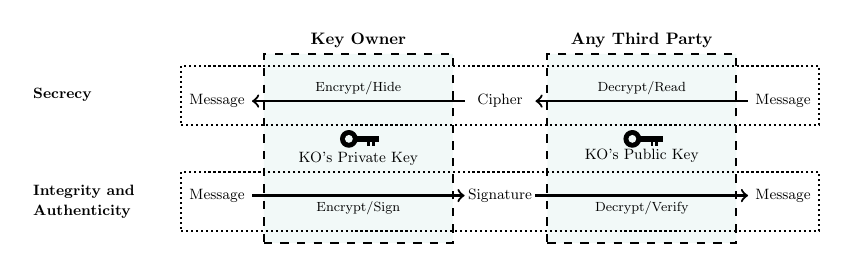
\begin{tikzpicture}[domain=-6:12,scale=0.6, every node/.style={scale=0.6}]
	
	\draw[fill= highlight!15, draw=black, thick, dashed] (0,0) -- (4,0) -- (4,4) -- (0,4) -- (0,0);
	\draw[fill= highlight!15, draw=black, thick, dashed] (6,0) -- (10,0) -- (10,4) -- (6,4) -- (6,0);
	
	\draw[draw=black, thick, densely dotted] (-1.75,2.5) -- (11.75,2.5) -- (11.75,3.75) -- (-1.75,3.75) -- (-1.75,2.5) node[left,midway,text width=3cm]{\small{\textbf{Secrecy}}};
	\draw[draw=black, thick, densely dotted] (-1.75,0.25) -- (11.75,0.25) -- (11.75,1.5) -- (-1.75,1.5) -- (-1.75,0.25)node[left,midway,text width=3cm]{\small{\textbf{Integrity and\\ Authenticity}}};
	
	
	
	\draw[<-,thick] (-0.25,3) -- (4.25,3) node[above, midway] {\footnotesize{Encrypt/Hide}};
	\draw[<-,thick] (5.75,3) -- (10.25,3) node[above, midway] {\footnotesize{Decrypt/Read}};
	
	\draw[->,thick] (-0.25,1) -- (4.25,1) node[below, midway] {\footnotesize{Encrypt/Sign}} ;
	\draw[->,thick] (5.75,1) -- (10.25,1) node[below, midway] {\footnotesize{Decrypt/Verify}} ;
	
	
	%\draw[<-,thick] (-0.3,3) -- node[above] {\footnotesize{Entschlüsselung}} ++(4.6,0);
	%\draw[<-,thick] (5.7,3) -- node[above] {\footnotesize{Verschlüsselung}} ++(4.6,0);
	
	%\draw[->,thick] (-0.3,1) -- node[below] {\footnotesize{Verschlüsseln/Signatur}} ++(4.6,0);
	%\draw[->,thick] (5.7,1) -- node[below] {\footnotesize{Entschlüsseln/Kontrolle}} ++(4.6,0);
	
	\draw  plot (5,3) node[]{\small{Cipher}};
	\draw  plot (5,1) node[]{\small{Signature}};
	
	\draw  plot (-0.99,3) node[]{\small{Message}};
	\draw  plot (-0.99,1) node[]{\small{Message}};
	
	\draw  plot (10.99,3) node[]{\small{Message}};
	\draw  plot (10.99,1) node[]{\small{Message}};
	
	%private key
	\filldraw[color=black] (1.8,2.2) circle (5pt) ;
	\filldraw[color=highlight!15] (1.8,2.2) circle (2pt);
	\filldraw[yshift=-0.05cm, xshift=0.1cm,color = black] (1.8,2.2) rectangle ++(15pt,3pt) ;
	\filldraw[yshift=-0.13cm, xshift=0.4cm,color = black] (1.8,2.2) rectangle ++(1pt,4pt) ;
	\filldraw[yshift=-0.13cm, xshift=0.5cm,color = black] (1.8,2.2) rectangle ++(1pt,4pt) ;
	\draw[color=black] plot (2,2.05) node[below] {\small{KO's Private Key}};
	\draw[color=black] plot (2,4) node[above] {\textbf{Key Owner}};
	
	%public key
	\filldraw[color=black] (7.8,2.2) circle (5pt);
	\filldraw[color=highlight!15] (7.8,2.2) circle (2pt);
	\filldraw[yshift=-0.05cm, xshift=0.1cm,color = black] (7.8,2.2) rectangle ++(15pt,3pt) ;
	\filldraw[yshift=-0.13cm, xshift=0.4cm,color = black] (7.8,2.2) rectangle ++(1pt,4pt) ;
	\filldraw[yshift=-0.13cm, xshift=0.5cm,color = black] (7.8,2.2) rectangle ++(1pt,4pt) ;
	\draw[color=black] plot (8,2.1) node[below] {\small{KO's Public Key}};
	\draw[color=black] plot (8,4) node[above] {\textbf{Any Third Party}};
	
\end{tikzpicture}
\end{frame}
%%%


%%%
\begin{frame}{Transaction Legitimacy}
	\begin{figure}[h!]
		\center
		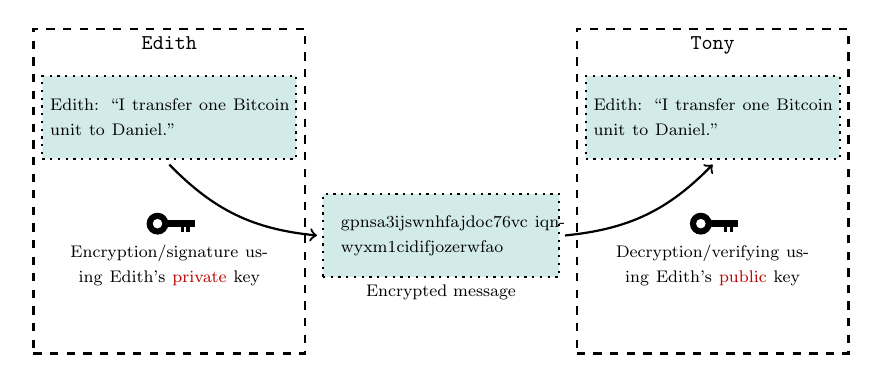
\begin{tikzpicture}[domain=-8:8,scale=0.75, every node/.style={scale=0.76}]

\draw[dashed,thick] (-3.3,0) -- (1.3,0) -- (1.3,5.5) -- (-3.3,5.5) node[midway,below]{\texttt{Edith}}--(-3.3,0);

\filldraw[fill=highlight!50,dotted,thick] (-3.15,3.3) -- (1.15,3.3) -- (1.15,4.7) -- (-3.15,4.7) -- (-3.15,3.3) node[midway, right=0.0cm ,text width=4.1cm]{\footnotesize{Edith: ``I transfer one  Bitcoin unit to Daniel.''}};

\draw[->,thick] (-1,3.2) to[bend right = 20] (1.5,2);

\draw[dashed,thick] (5.9,0) -- (10.5,0) -- (10.5,5.5) -- (5.9,5.5) node[midway,below]{\texttt{Tony}}--(5.9,0);

\filldraw[fill=highlight!50,dotted,thick] (6.05,3.3) -- (10.35,3.3) -- (10.35,4.7) -- (6.05,4.7) -- (6.05,3.3) node[midway, right=0.0cm ,text width=4.1cm]{\footnotesize{Edith: ``I transfer one Bitcoin unit to Daniel.''}};

\draw[->,thick] (5.7,2) to[bend right = 20] (8.2,3.2);

\filldraw[fill=highlight!50,dotted,thick] (1.6,1.3) -- (5.6,1.3) node[midway,below]{\footnotesize{Encrypted message}}-- (5.6,2.7) -- (1.6,2.7) -- (1.6,1.3) node[midway, right=0.13cm ,text width=4cm]{\footnotesize{gpnsa3ijswnhfajdoc76vc iqnwyxm1cidifjozerwfao}};

%private key
  \filldraw[color=black] (-1.2,2.2) circle (5pt);
  \filldraw[color=white!15] (-1.2,2.2) circle (2pt);
  \filldraw[yshift=-0.05cm, xshift=0.1cm,color = black] (-1.2,2.2) rectangle ++(15pt,3pt) ;
  \filldraw[yshift=-0.13cm, xshift=0.4cm,color = black] (-1.2,2.2) rectangle ++(1pt,4pt) ;
  \filldraw[yshift=-0.13cm, xshift=0.5cm,color = black] (-1.2,2.2) rectangle ++(1pt,4pt) ;
  \draw[color=black] plot (-1,2.1)                  node[align=center,below=0.1cm, text width= 4.5cm] {\footnotesize{Encryption/signature using Edith's  \color{focus} private \color{black} key}};

%public key
  \filldraw[color=black] (8,2.2) circle (5pt);
  \filldraw[color=white!15] (8,2.2) circle (2pt);
  \filldraw[yshift=-0.05cm, xshift=0.1cm,color = black] (8,2.2) rectangle ++(15pt,3pt) ;
  \filldraw[yshift=-0.13cm, xshift=0.4cm,color = black] (8,2.2) rectangle ++(1pt,4pt) ;
  \filldraw[yshift=-0.13cm, xshift=0.5cm,color = black] (8,2.2) rectangle ++(1pt,4pt) ;
  \draw[color=black] plot (8.2,2.1)                  node[align=center,below=0.1cm, text width= 4.5cm] {\footnotesize{Decryption/verifying using Edith's \color{focus} public \color{black}key}};

\end{tikzpicture}

		\caption*{Encryption and decryption of the transaction message}
		\label{fig:asymmeinfach}
	\end{figure}
\end{frame}
%%%

%%%
\begin{frame}{Transaction Consensus}
\textbf{Goal: }Deciding which (legitimate) transactions are valid. \\
\vspace{1em}
\uncover<2->{
Potential Problem: Assume both transactions have valid signatures, but spend the same Bitcoin units. What now? \\
\begin{figure}[h!]
	\center
	\begin{figure}[h!]
\center
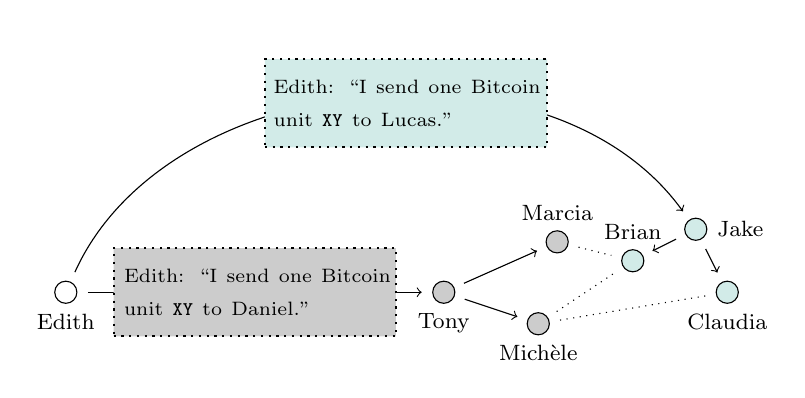
\begin{tikzpicture}[domain=-8:8, scale=0.8]
\coordinate (c1) at (0,0);
\coordinate (c2) at (6,0);
\coordinate (c3) at (7.8,0.8);
\coordinate (c4) at (7.5,-0.5);
\coordinate (c5) at (9,0.5);
\coordinate (c6) at (10,1);
\coordinate (c7) at (10.5,0);
\filldraw[draw=black,fill=white] (c1) circle (5pt) node[below=0.15cm,color=black]{\footnotesize{Edith}};
\filldraw[color=black,fill=black!20] (c2) circle (5pt) node[below=0.15cm,color=black]{\footnotesize{Tony}};
\filldraw[color=black,fill=black!20] (c3) circle (5pt) node[above=0.15cm,color=black]{\footnotesize{Marcia}};
\filldraw[color=black,fill=black!20] (c4) circle (5pt) node[below=0.15cm,color=black]{\footnotesize{Michèle}};
\filldraw[color=black,fill=highlight!50] (c5) circle (5pt) node[above=0.15cm,color=black]{\footnotesize{Brian}};
\filldraw[color=black,fill=highlight!50] (c6) circle (5pt) node[right=0.15cm,color=black]{\footnotesize{Jake}};
\filldraw[color=black,fill=highlight!50] (c7) circle (5pt) node[below=0.15cm,color=black]{\footnotesize{Claudia}};

\draw[shorten >=0.28cm,shorten <=0.28cm,->,color=black] (c1) to[bend left = 60] (c6);

\draw[shorten >=0.28cm,shorten <=0.28cm,->] (c1) to[] (c2);
\draw[shorten >=0.28cm,shorten <=0.28cm,->] (c2) to[] (c3);
\draw[shorten >=0.28cm,shorten <=0.28cm,->] (c2) to[] (c4);
\draw[shorten >=0.28cm,shorten <=0.28cm, dotted] (c3) to[] (c5);
\draw[shorten >=0.28cm,shorten <=0.28cm,dotted] (c4) to[] (c5);
\draw[shorten >=0.28cm,shorten <=0.28cm,dotted] (c4) to[] (c7);
\draw[shorten >=0.28cm,shorten <=0.28cm,->,color=black] (c6) to[] (c5);
\draw[shorten >=0.28cm,shorten <=0.28cm,->,color=black] (c6) to[] (c7);

\filldraw[fill=black!20,dotted,thick] (0.76,-0.7) -- (5.24,-0.7) -- (5.24,0.7) -- (0.76,0.7) -- (0.76,-0.7) node[midway, right=-0.0cm,text width=3.5cm]{\scriptsize{Edith: ``I send one Bitcoin unit \texttt{XY} to Daniel.''}};

\filldraw[fill=highlight!50,dotted,thick] (3.16,2.3) -- (7.64,2.3) -- (7.64,3.7) -- (3.16,3.7) -- (3.16,2.3) node[midway, right=-0.02cm,text width=3.5cm]{\scriptsize{Edith: ``I send one Bitcoin unit \texttt{XY} to Lucas.''}};

\end{tikzpicture}
\end{figure}
\end{figure}
}
\end{frame}
%%%

%%%
\begin{frame}{Blocks and the Blockchain}
Transactions are bundled into blocks. \\
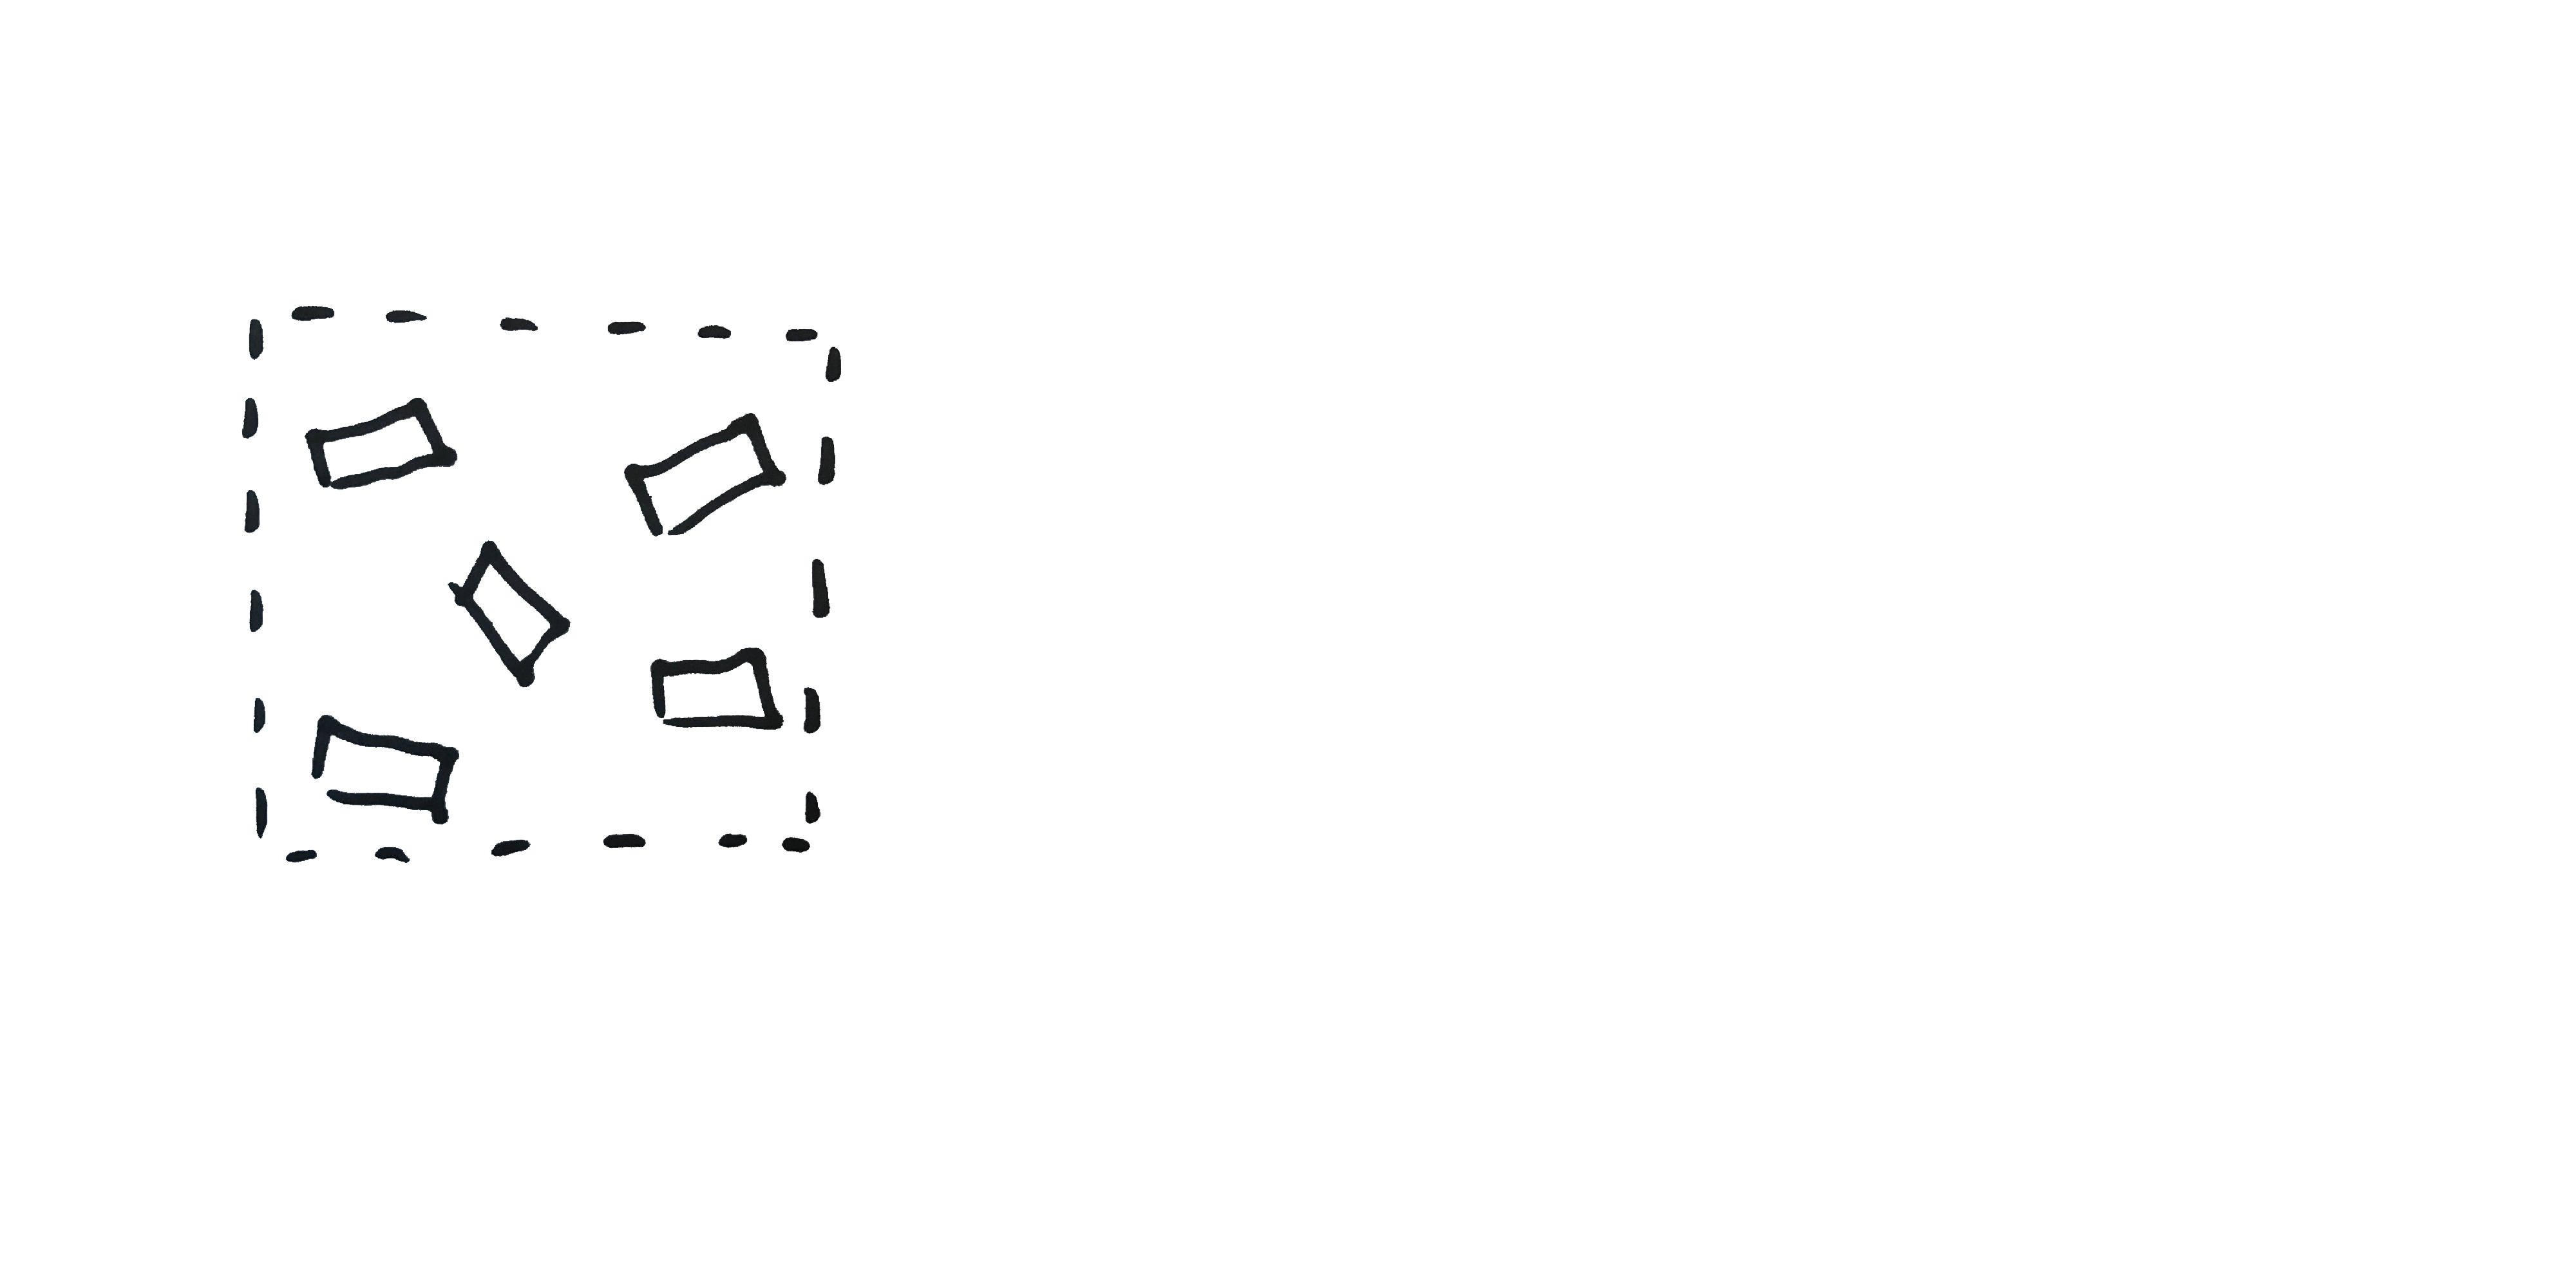
\includegraphics[width=6cm]{../assets/images/block_1.png} \\
\uncover<2->{
Blocks are sequentially linked $\rightarrow $ Blockchain \\
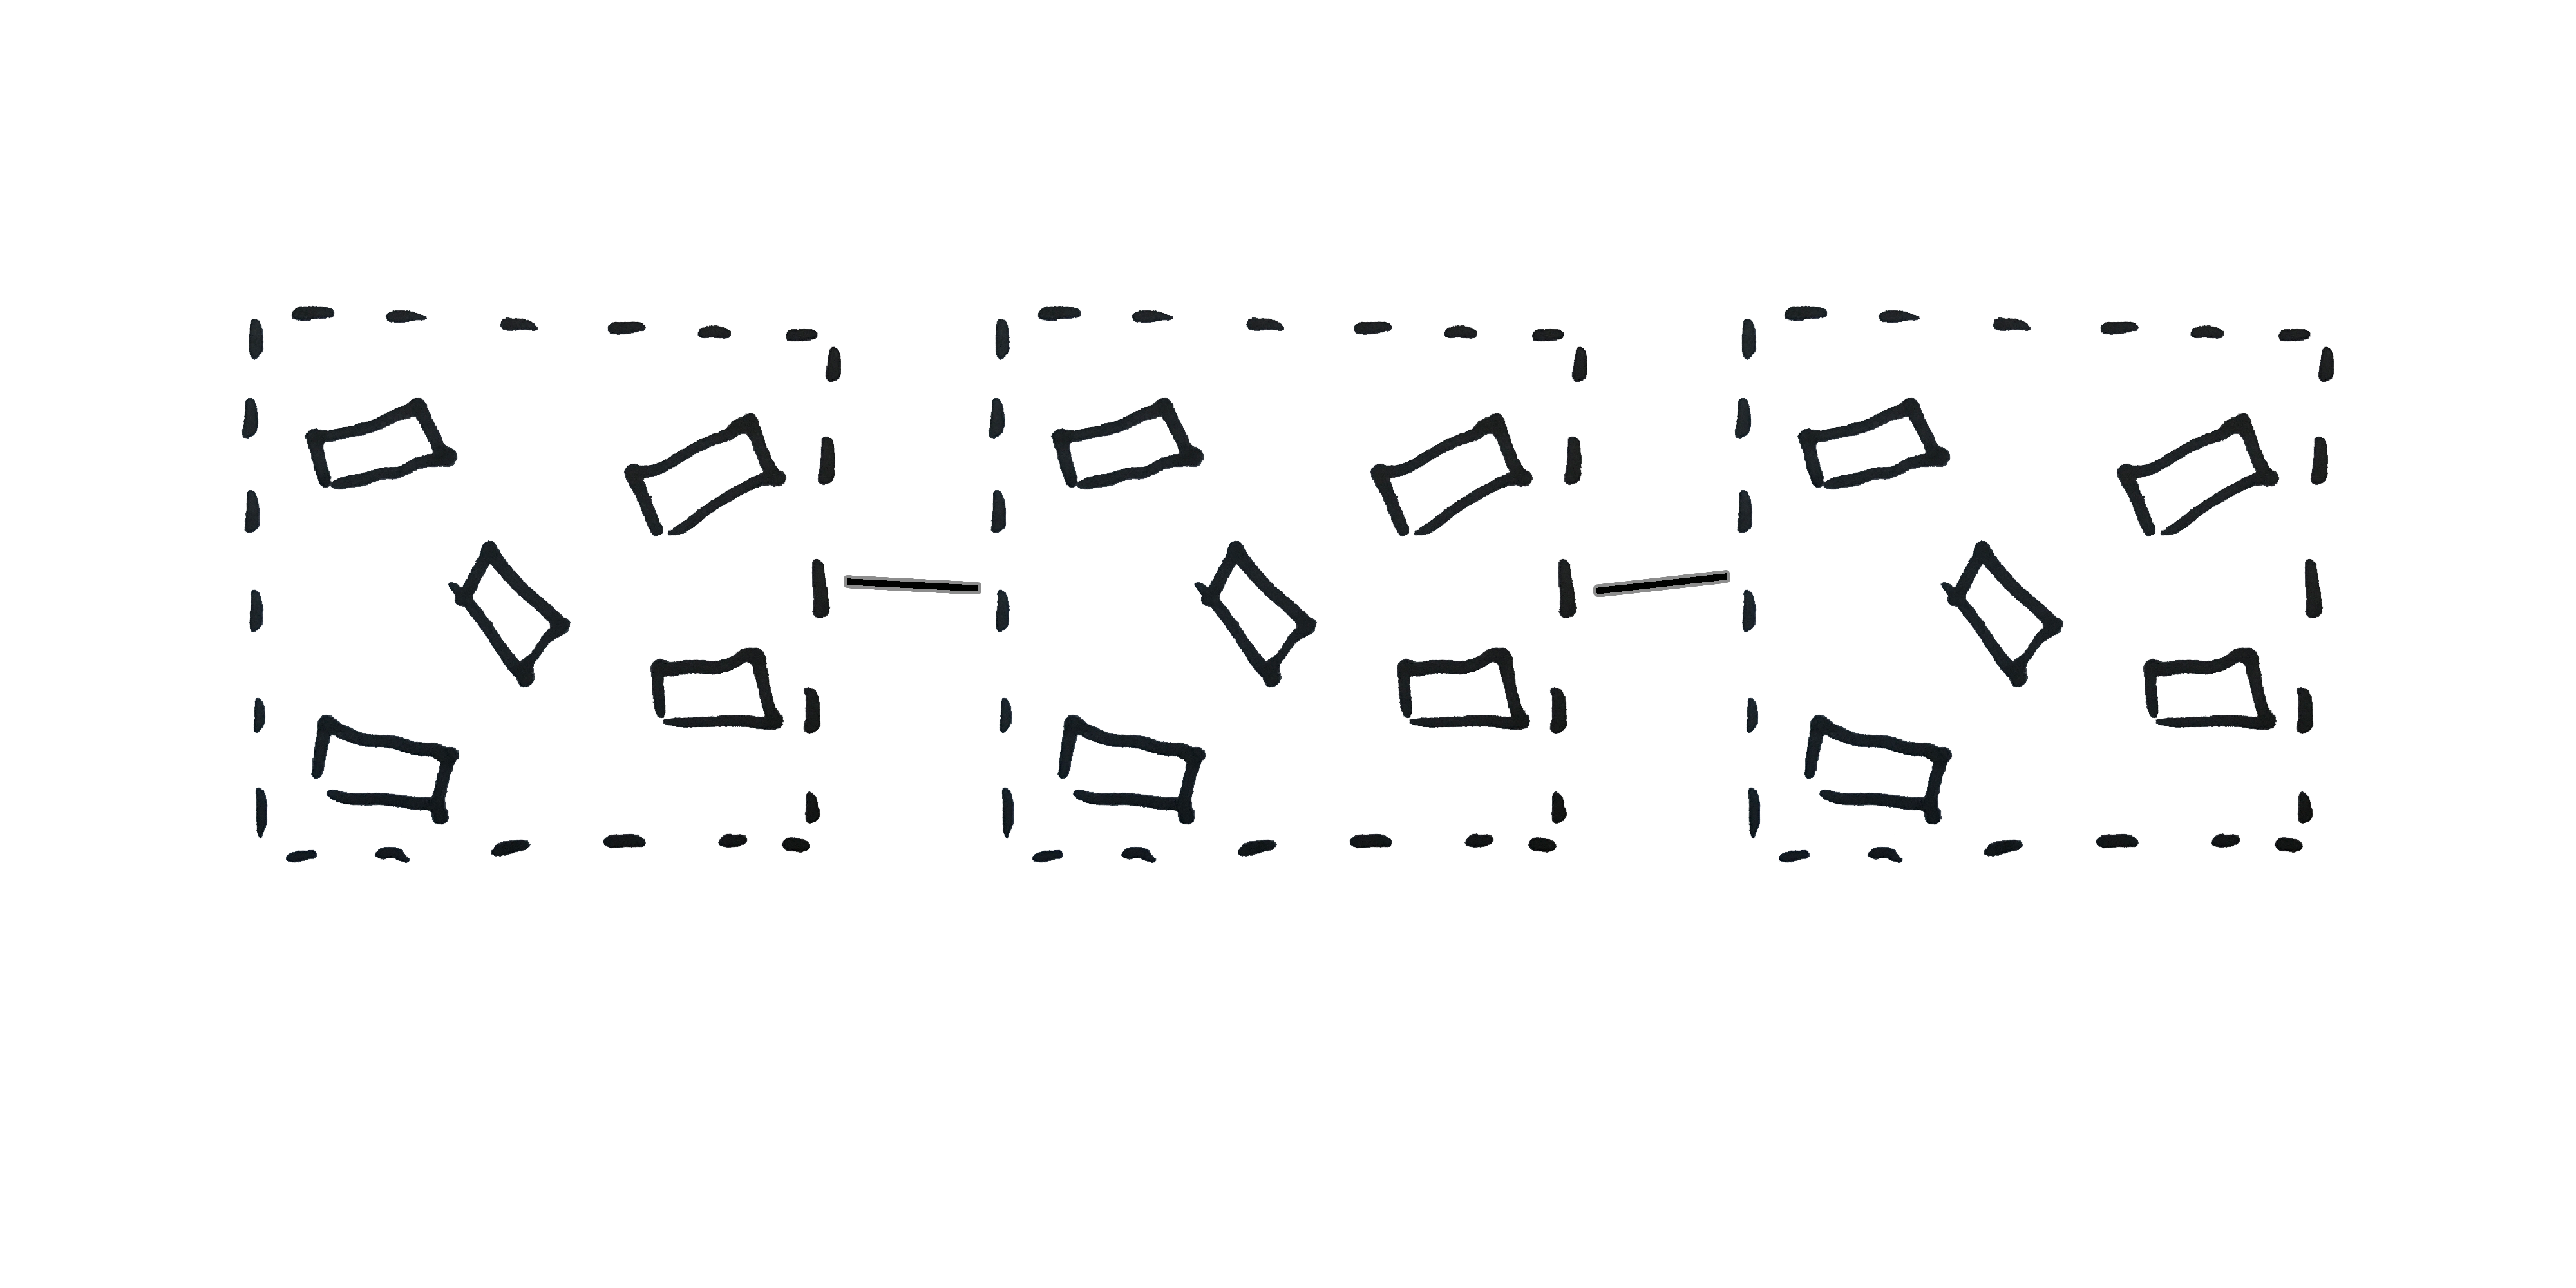
\includegraphics[width=6cm]{../assets/images/blocks_3.png}
}
\end{frame}
%%%


%%%
\begin{frame}{Bitcoin Mining}
Network participants, who assemble candidate blocks are usually referred to as Bitcoin Miners.
\center
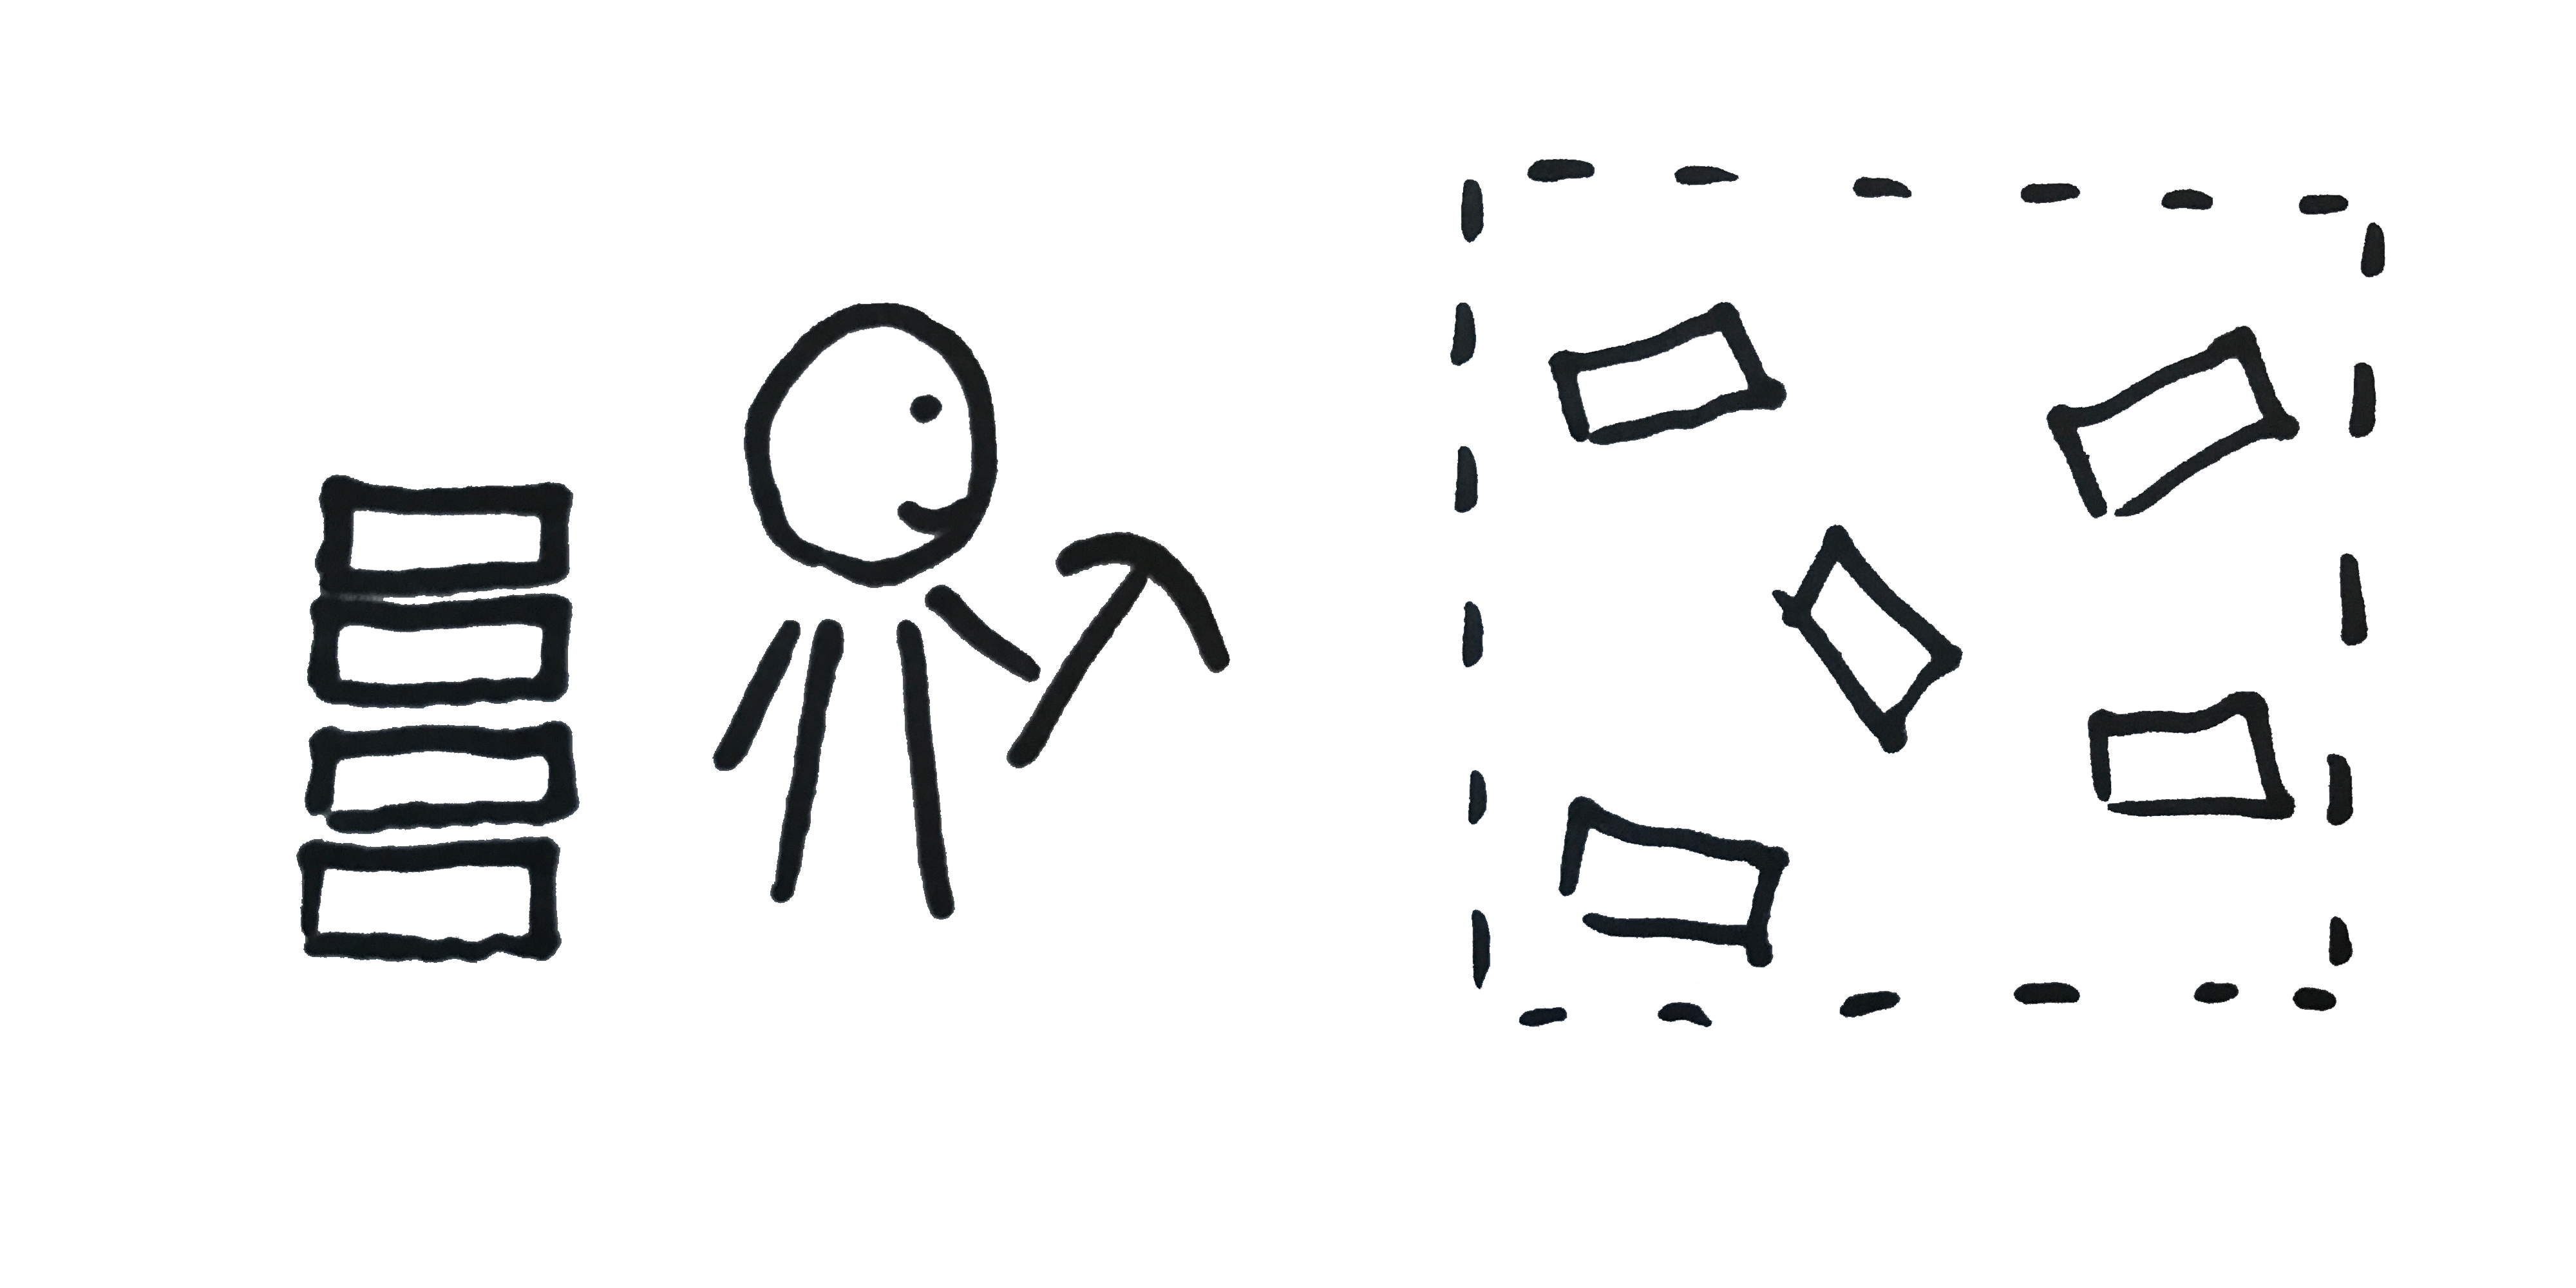
\includegraphics[width=6cm]{../assets/images/miner.png}
\uncover<2->{
	\begin{itemize}
	\item{Miner chooses the status quo on which to base its block. (Most recent version of Blockchain)}
}
\uncover<3->{
	\item{Miner chooses a subset of the transactions from its queue (mempool) to create a block, as long as they...}
	\begin{itemize}
		\item{\dots ...are legimitate.}
		\item{\dots ...do not conflict with other transactions.}
		\item{\dots do not exceed block size limitation.}
	\end{itemize}
	}
\end{itemize}
\end{frame}
%%%

%%%
\begin{frame}{Bitcoin Miner}
\center{
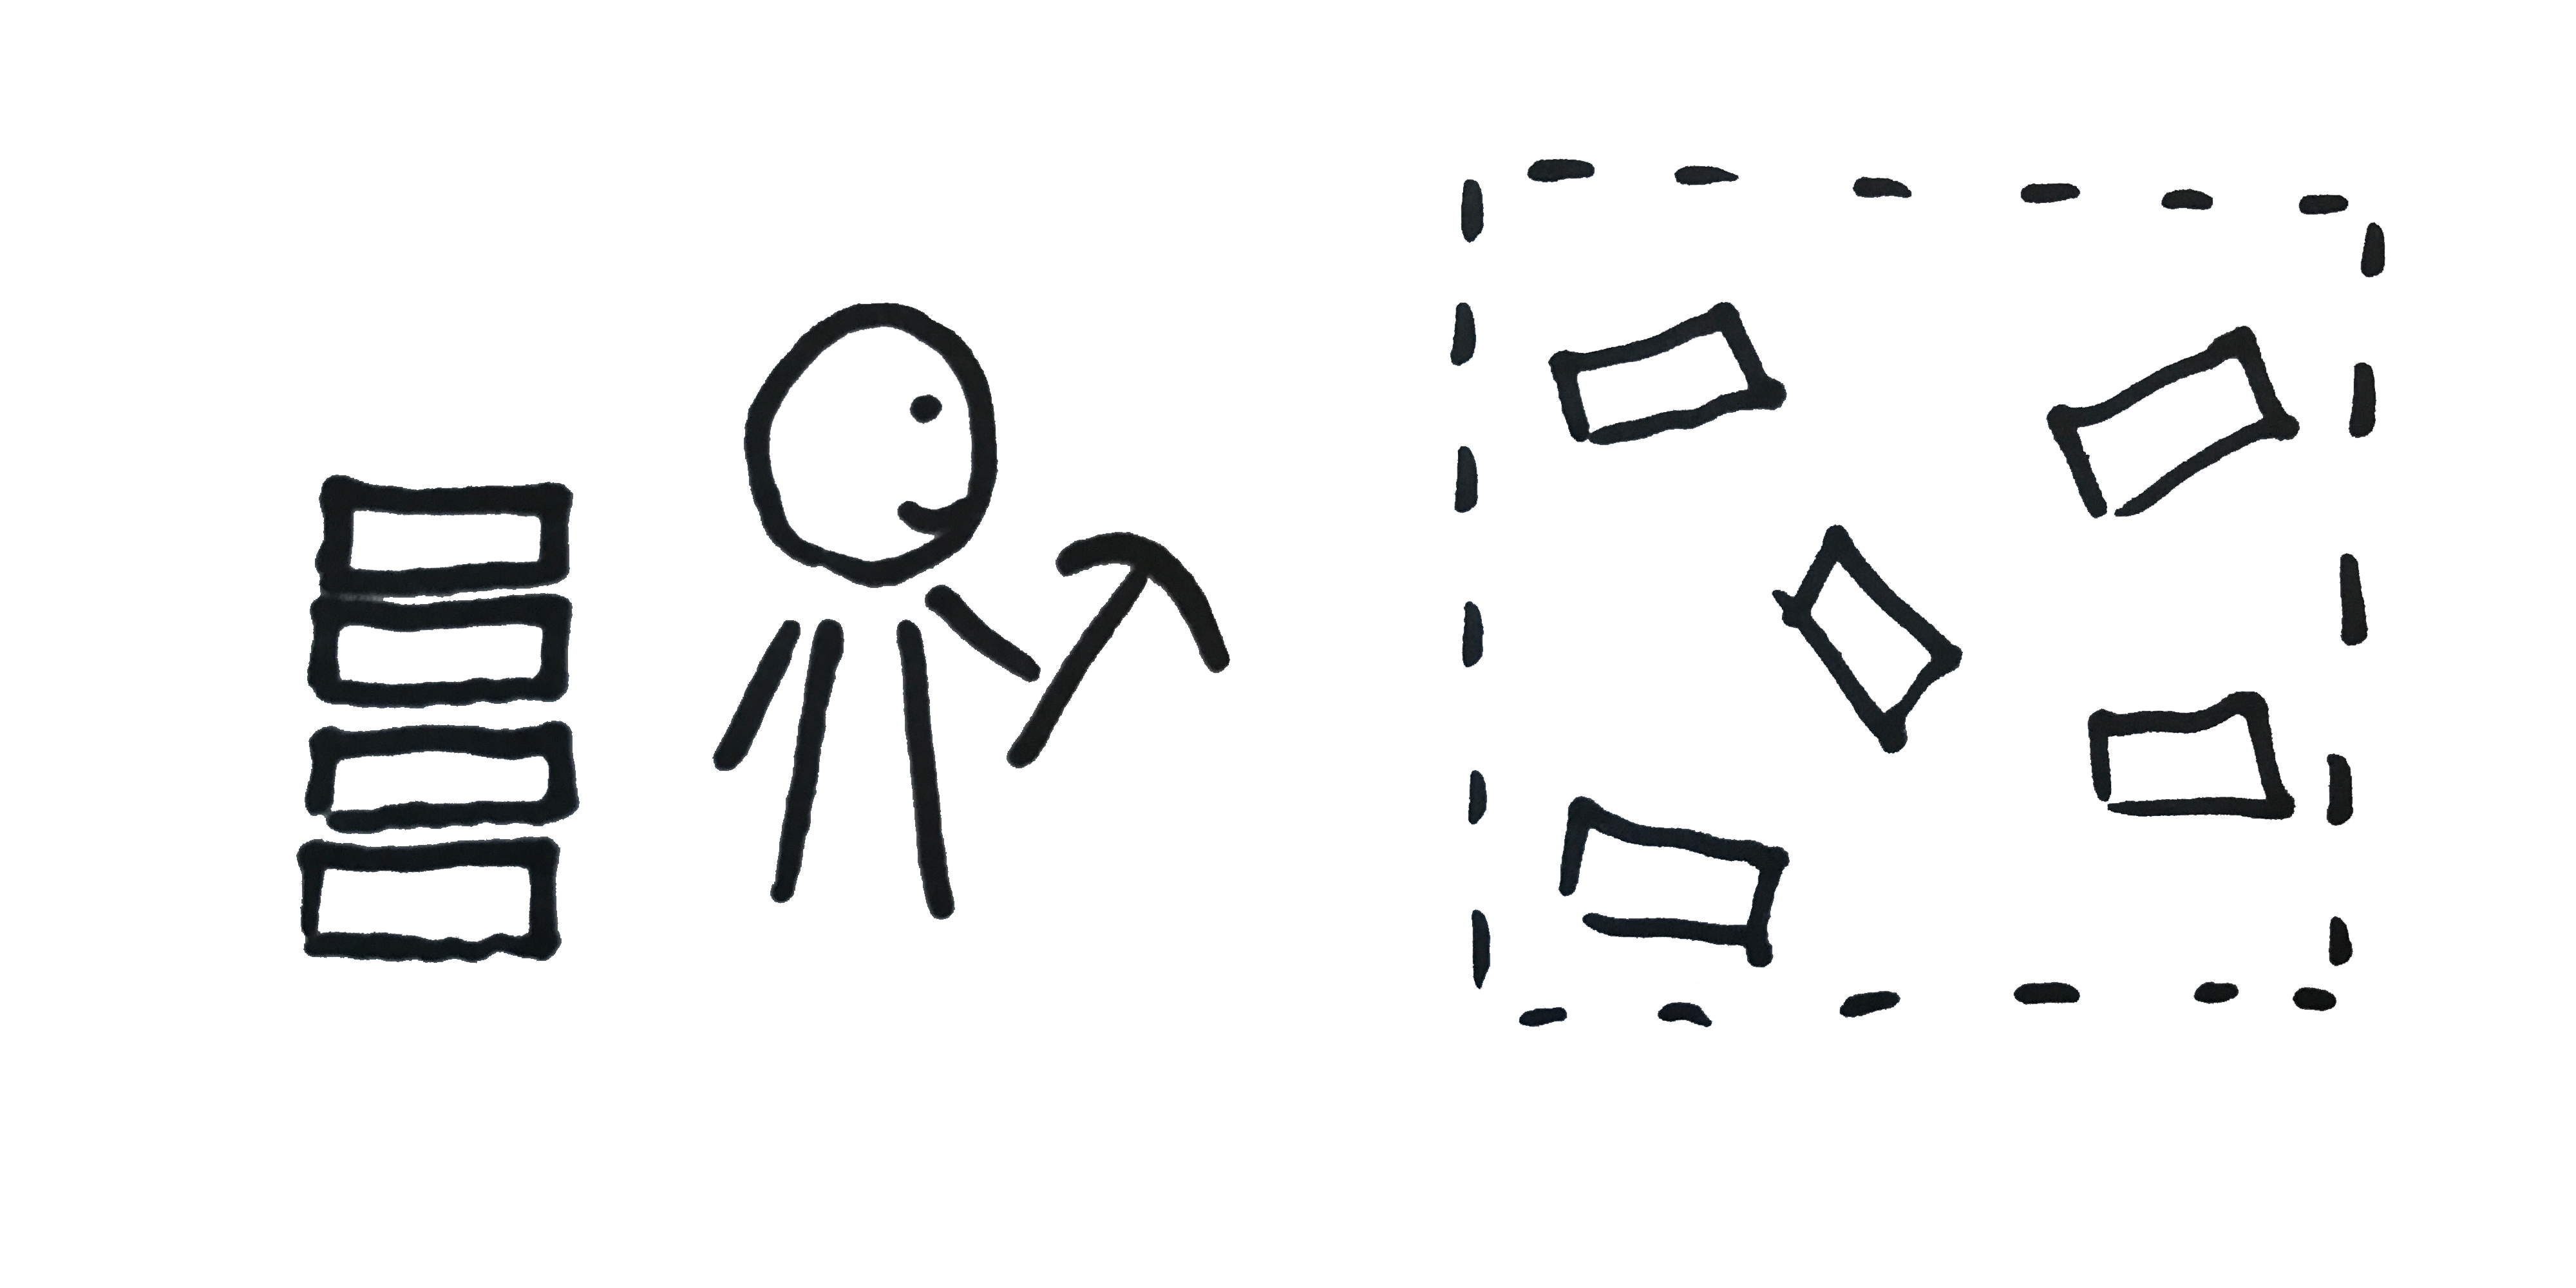
\includegraphics[width=4cm]{../assets/images/miner.png} \hspace{1cm} 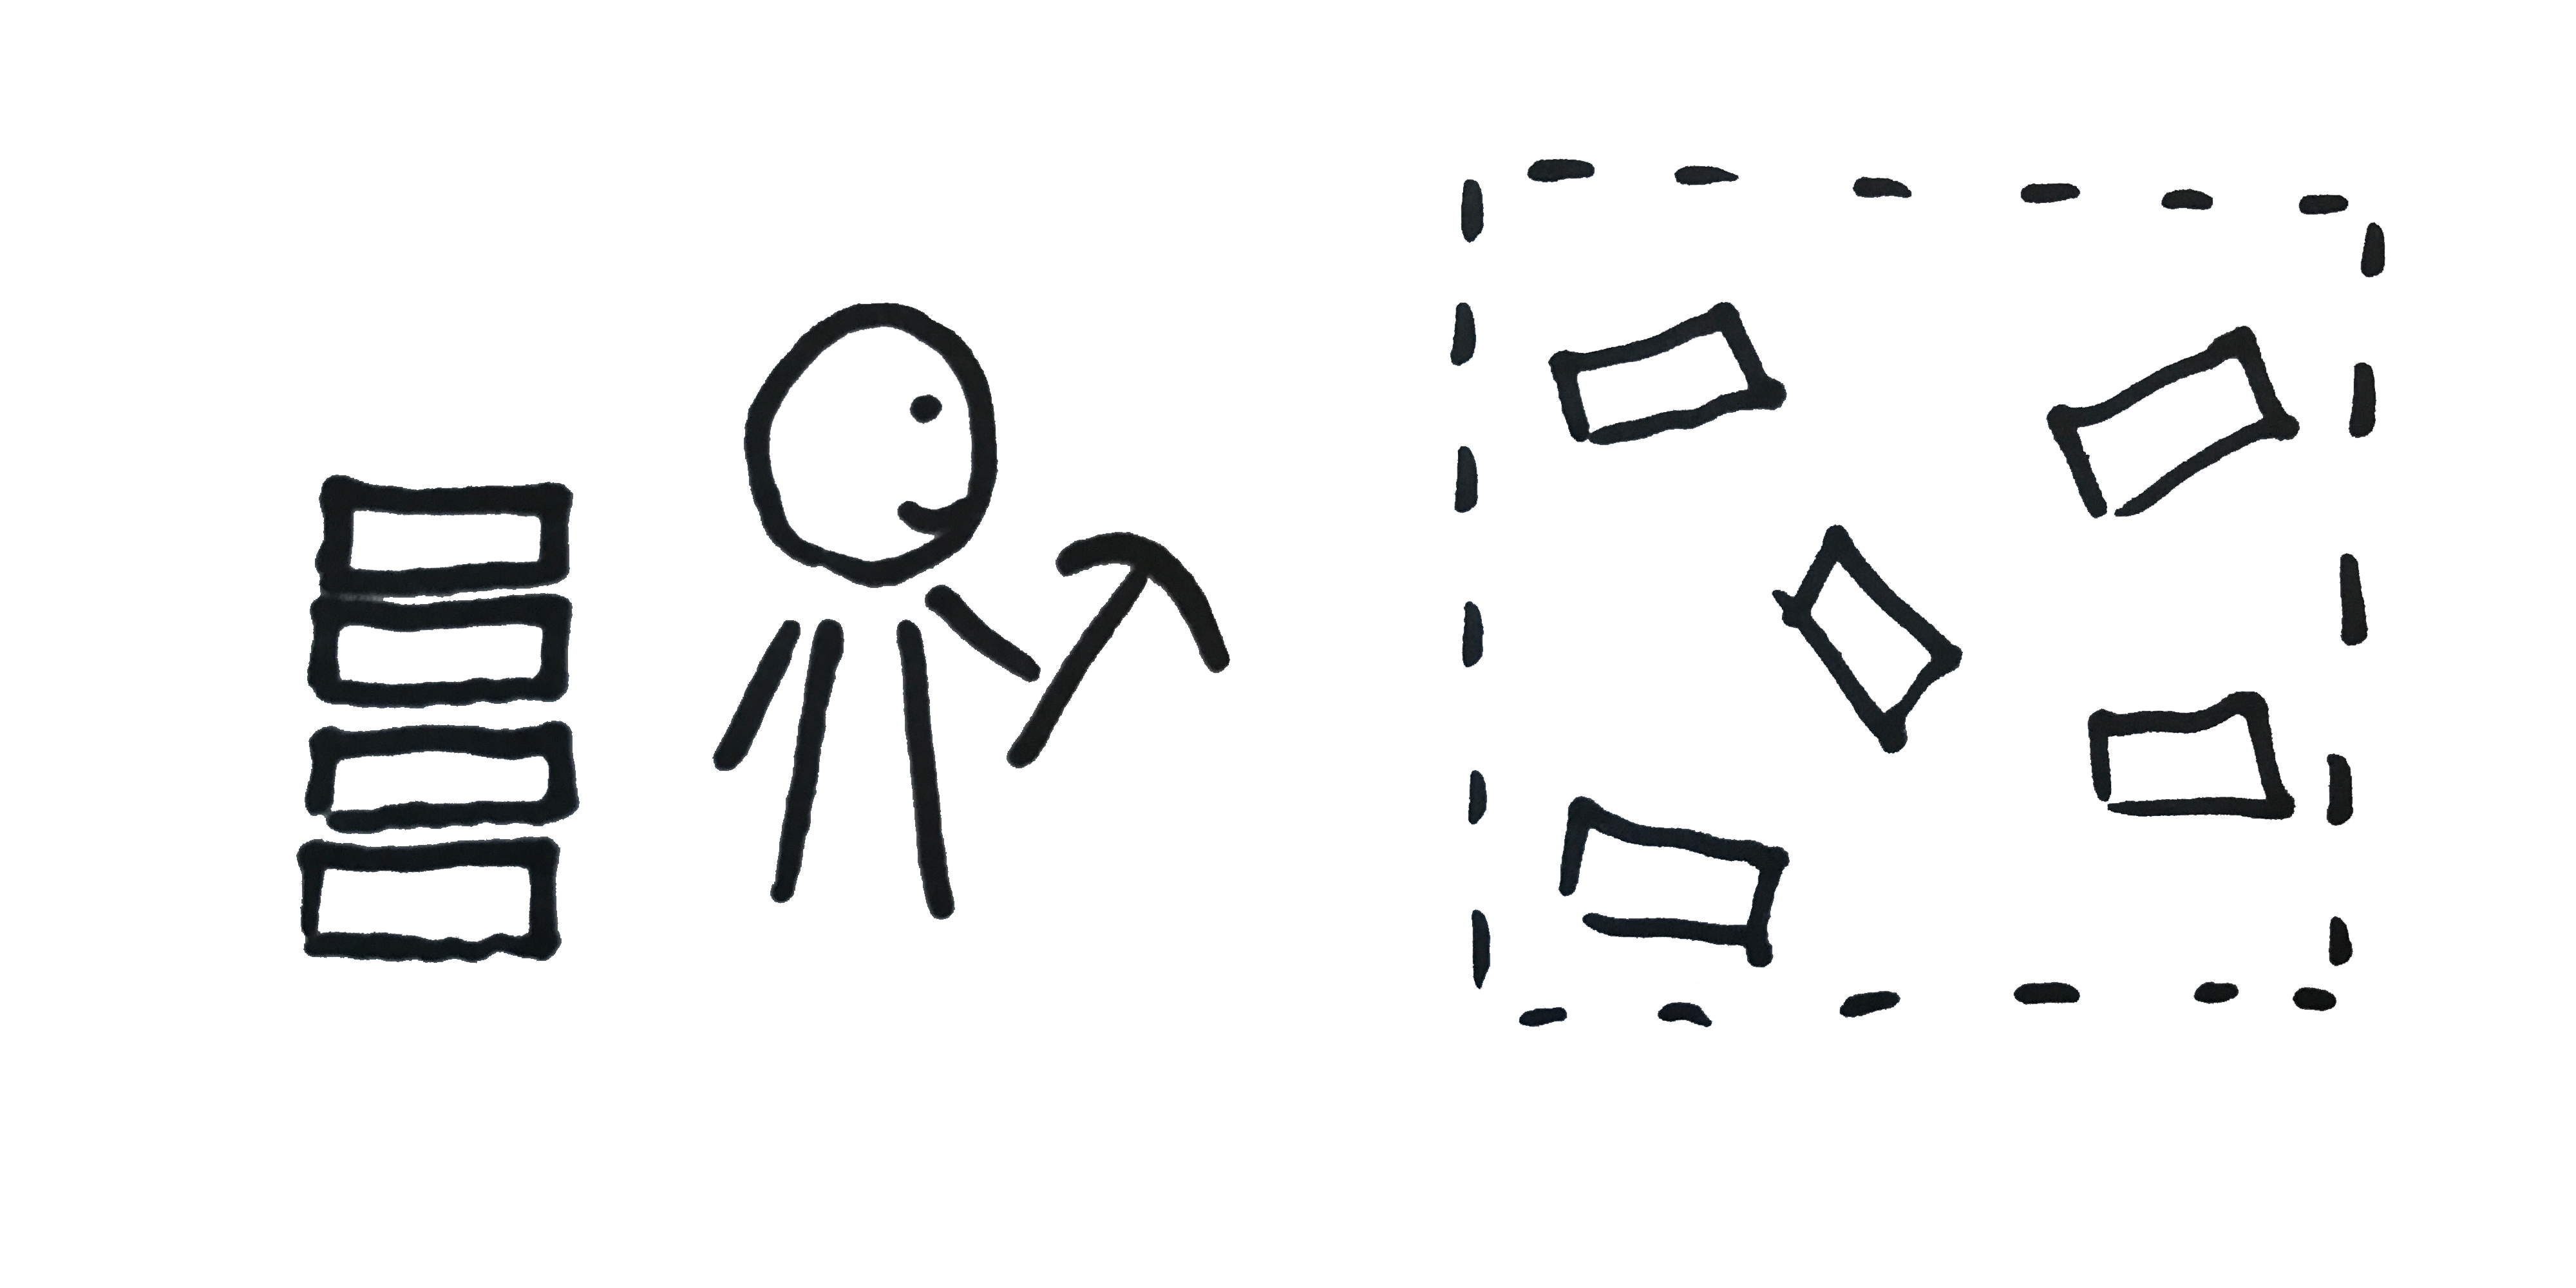
\includegraphics[width=4cm]{../assets/images/miner.png}\\
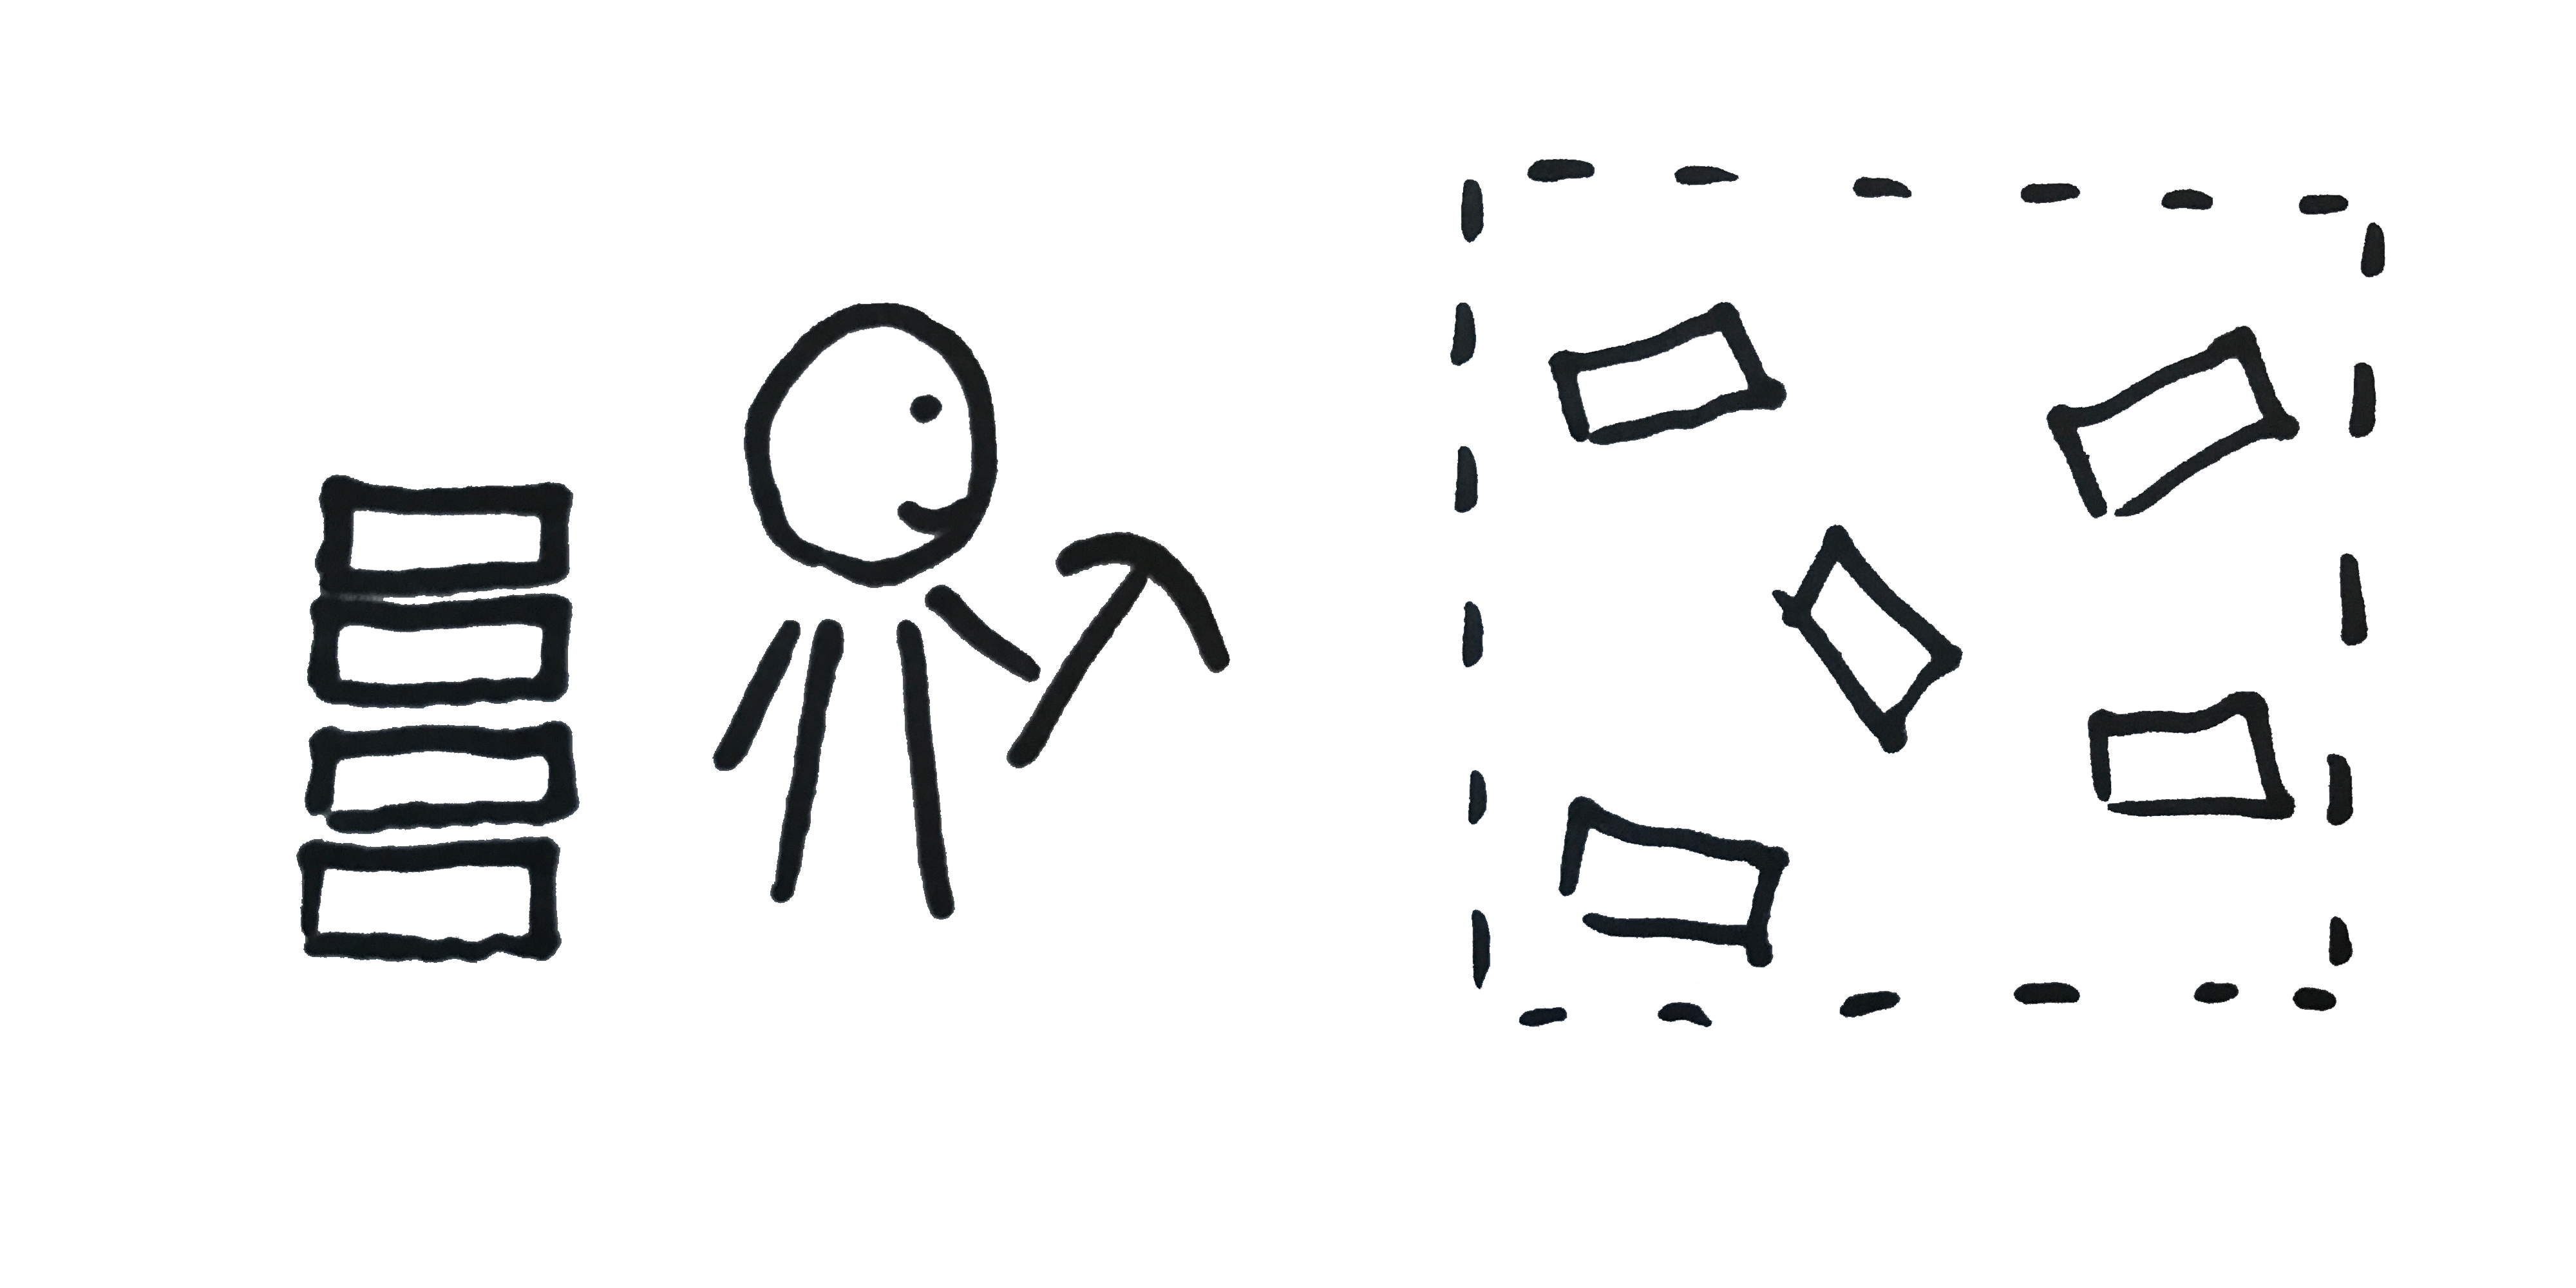
\includegraphics[width=4cm]{../assets/images/miner.png} \hspace{1cm} 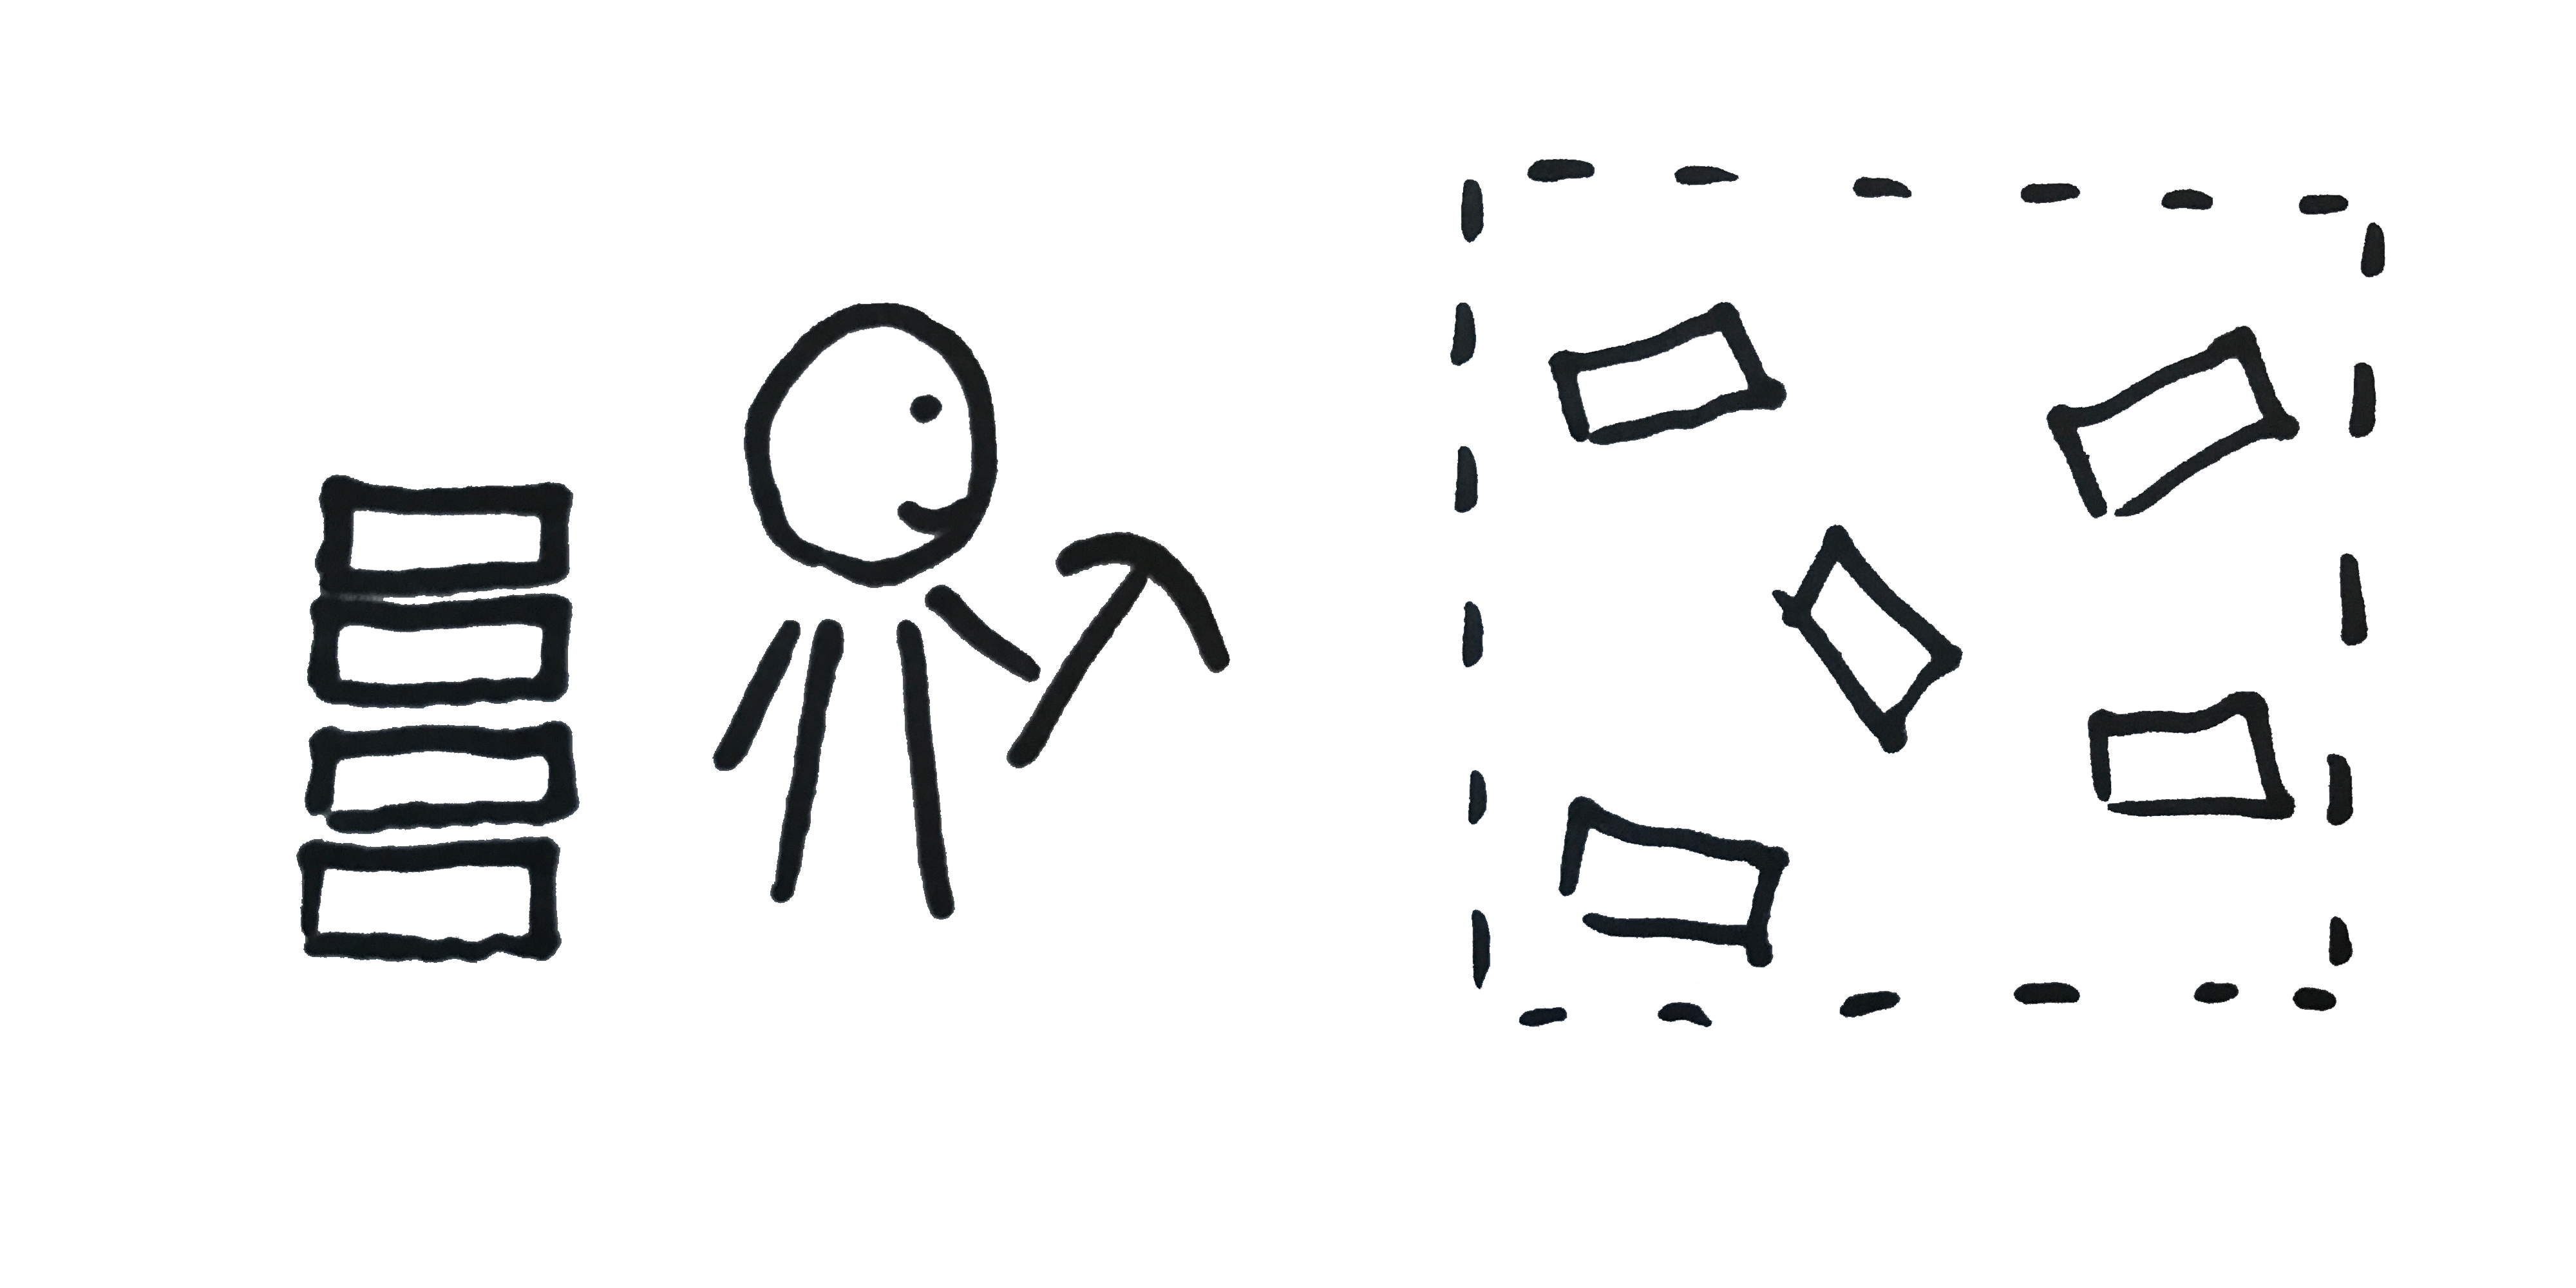
\includegraphics[width=4cm]{../assets/images/miner.png}\\
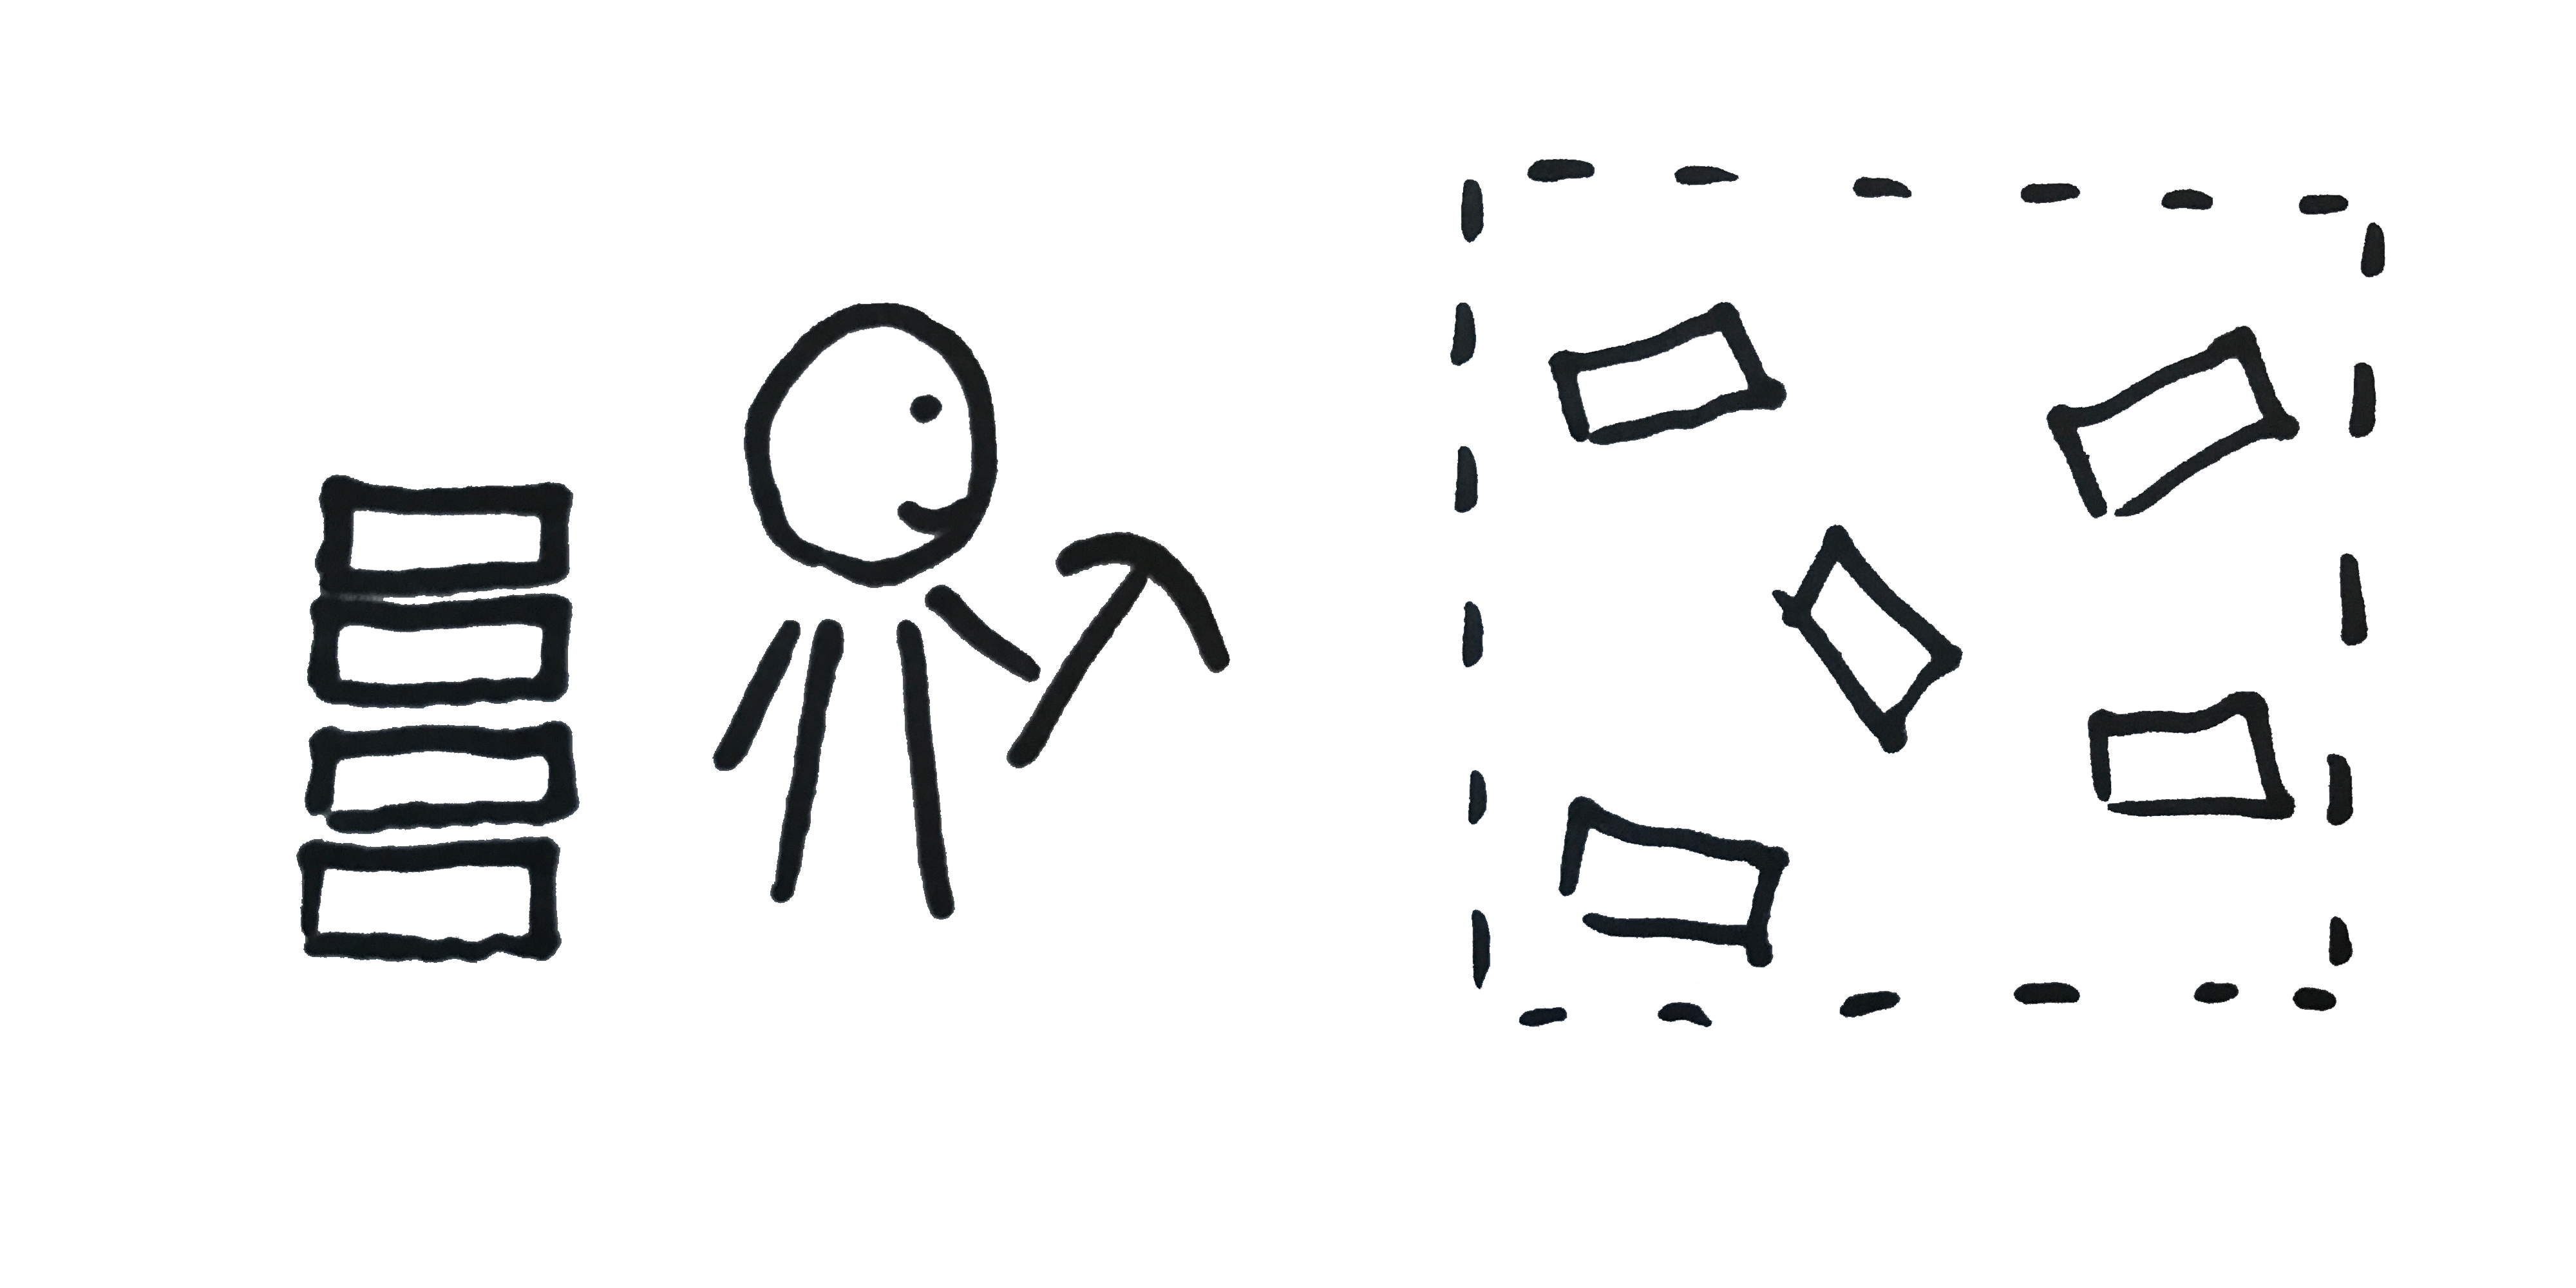
\includegraphics[width=4cm]{../assets/images/miner.png} \hspace{1cm} 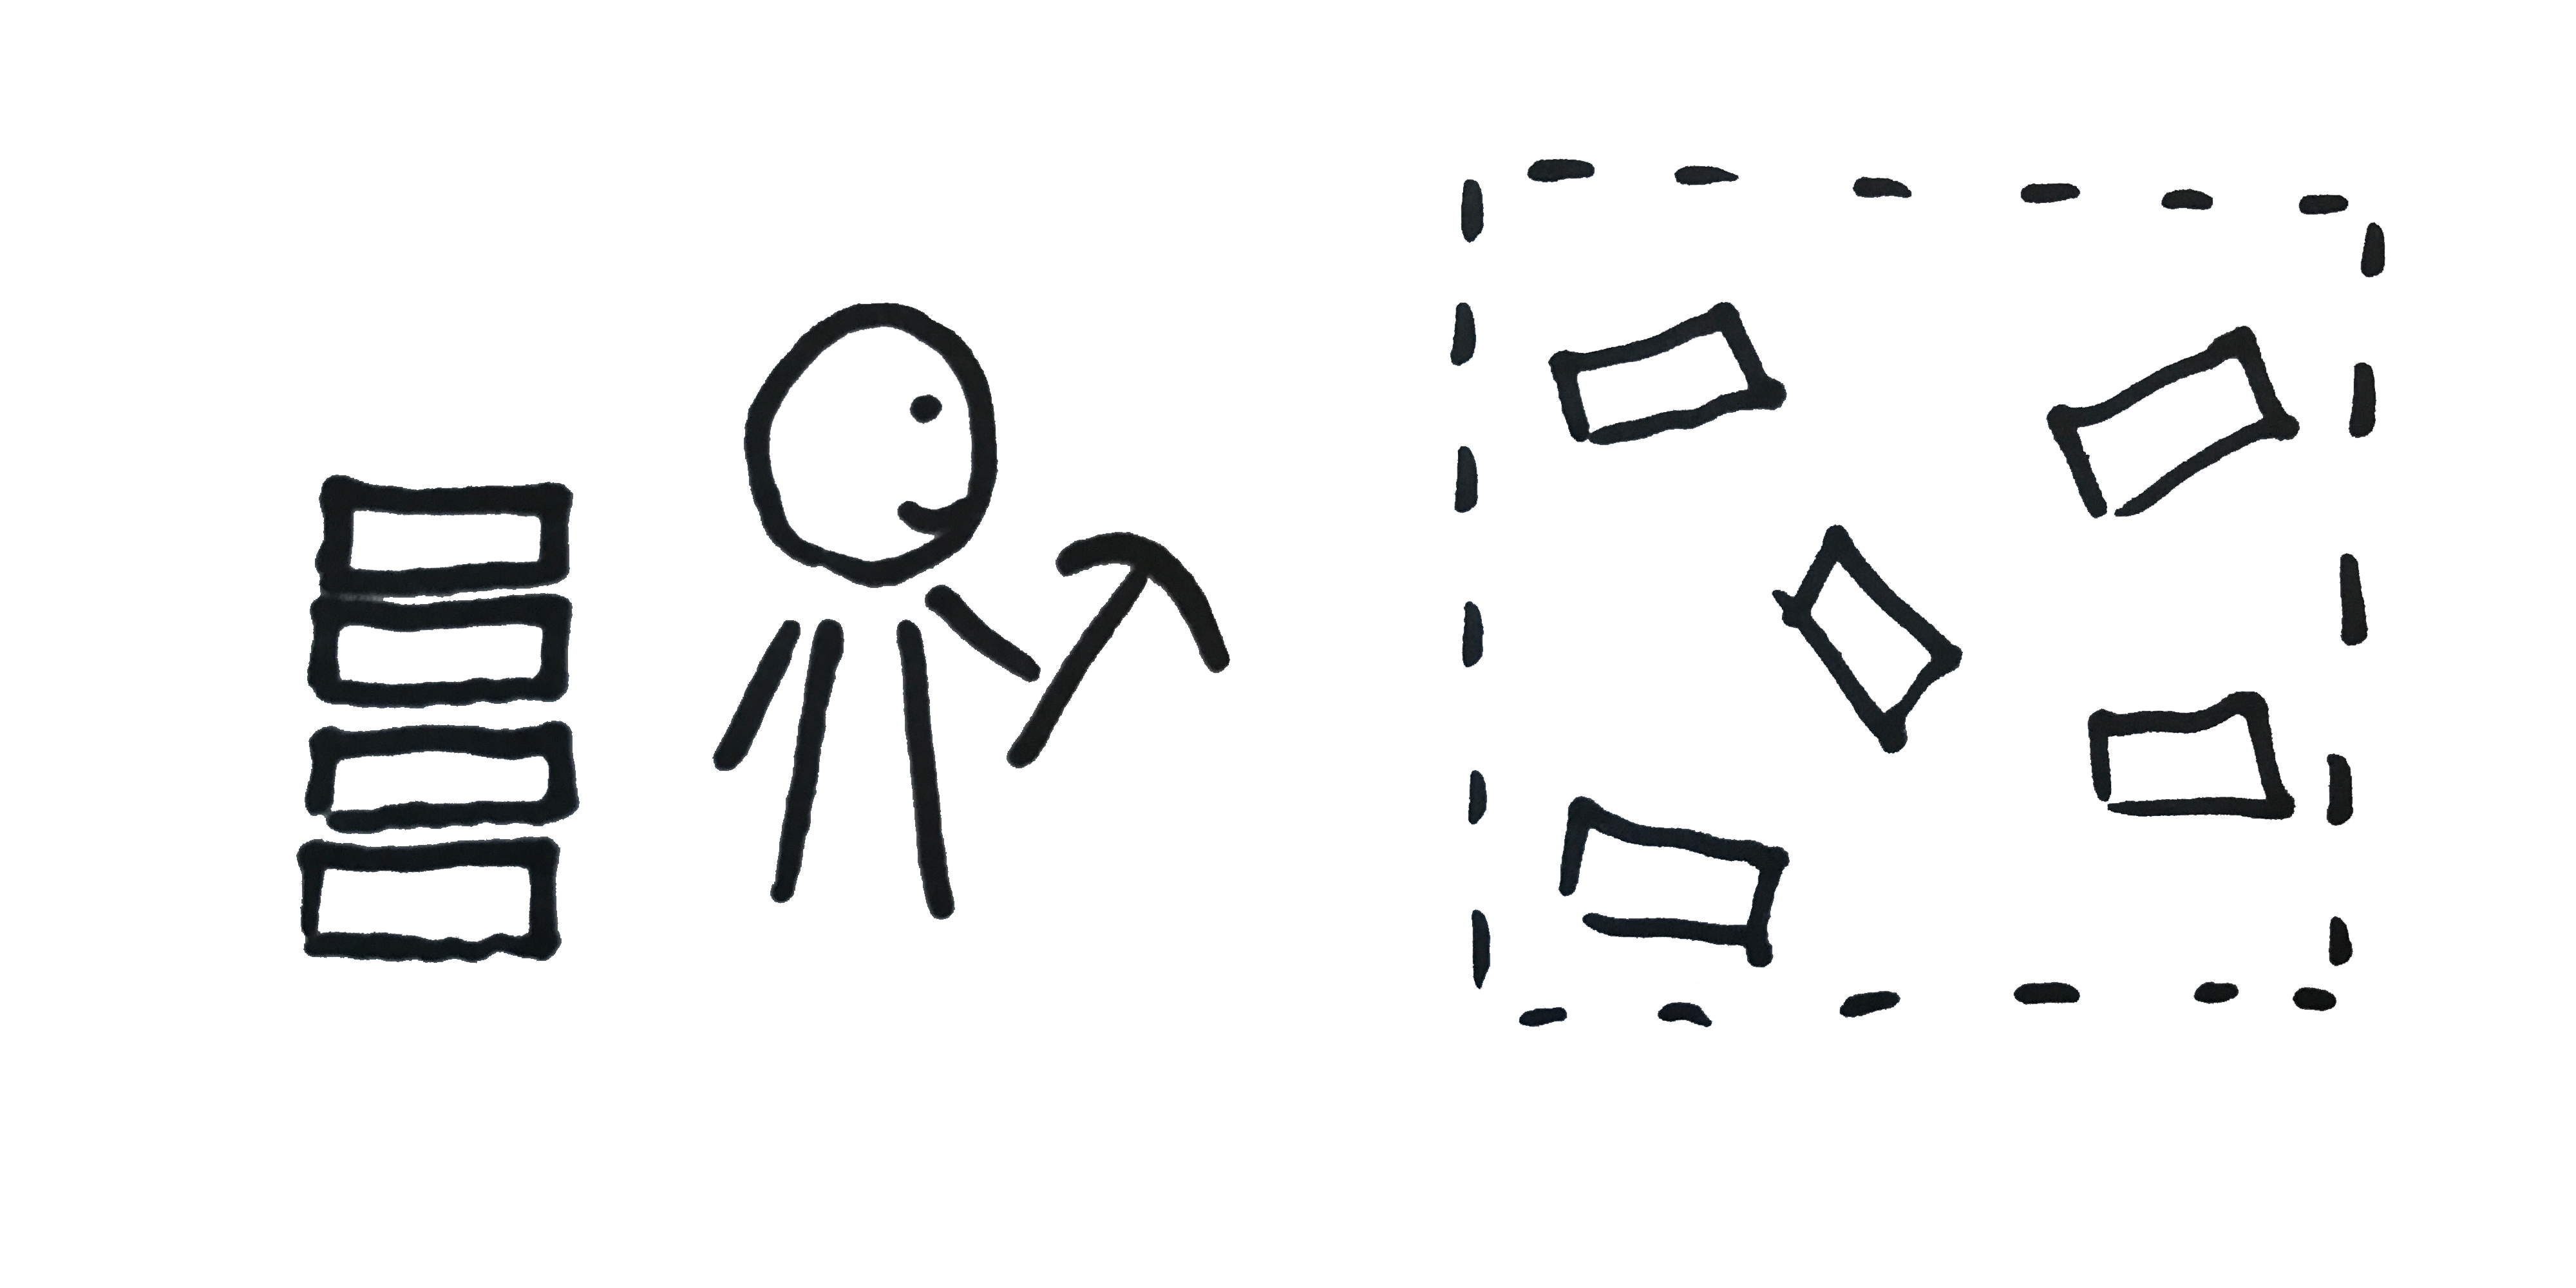
\includegraphics[width=4cm]{../assets/images/miner.png}\\
}
\end{frame}
%%%

%%%
\begin{frame}{Transaction Consensus}
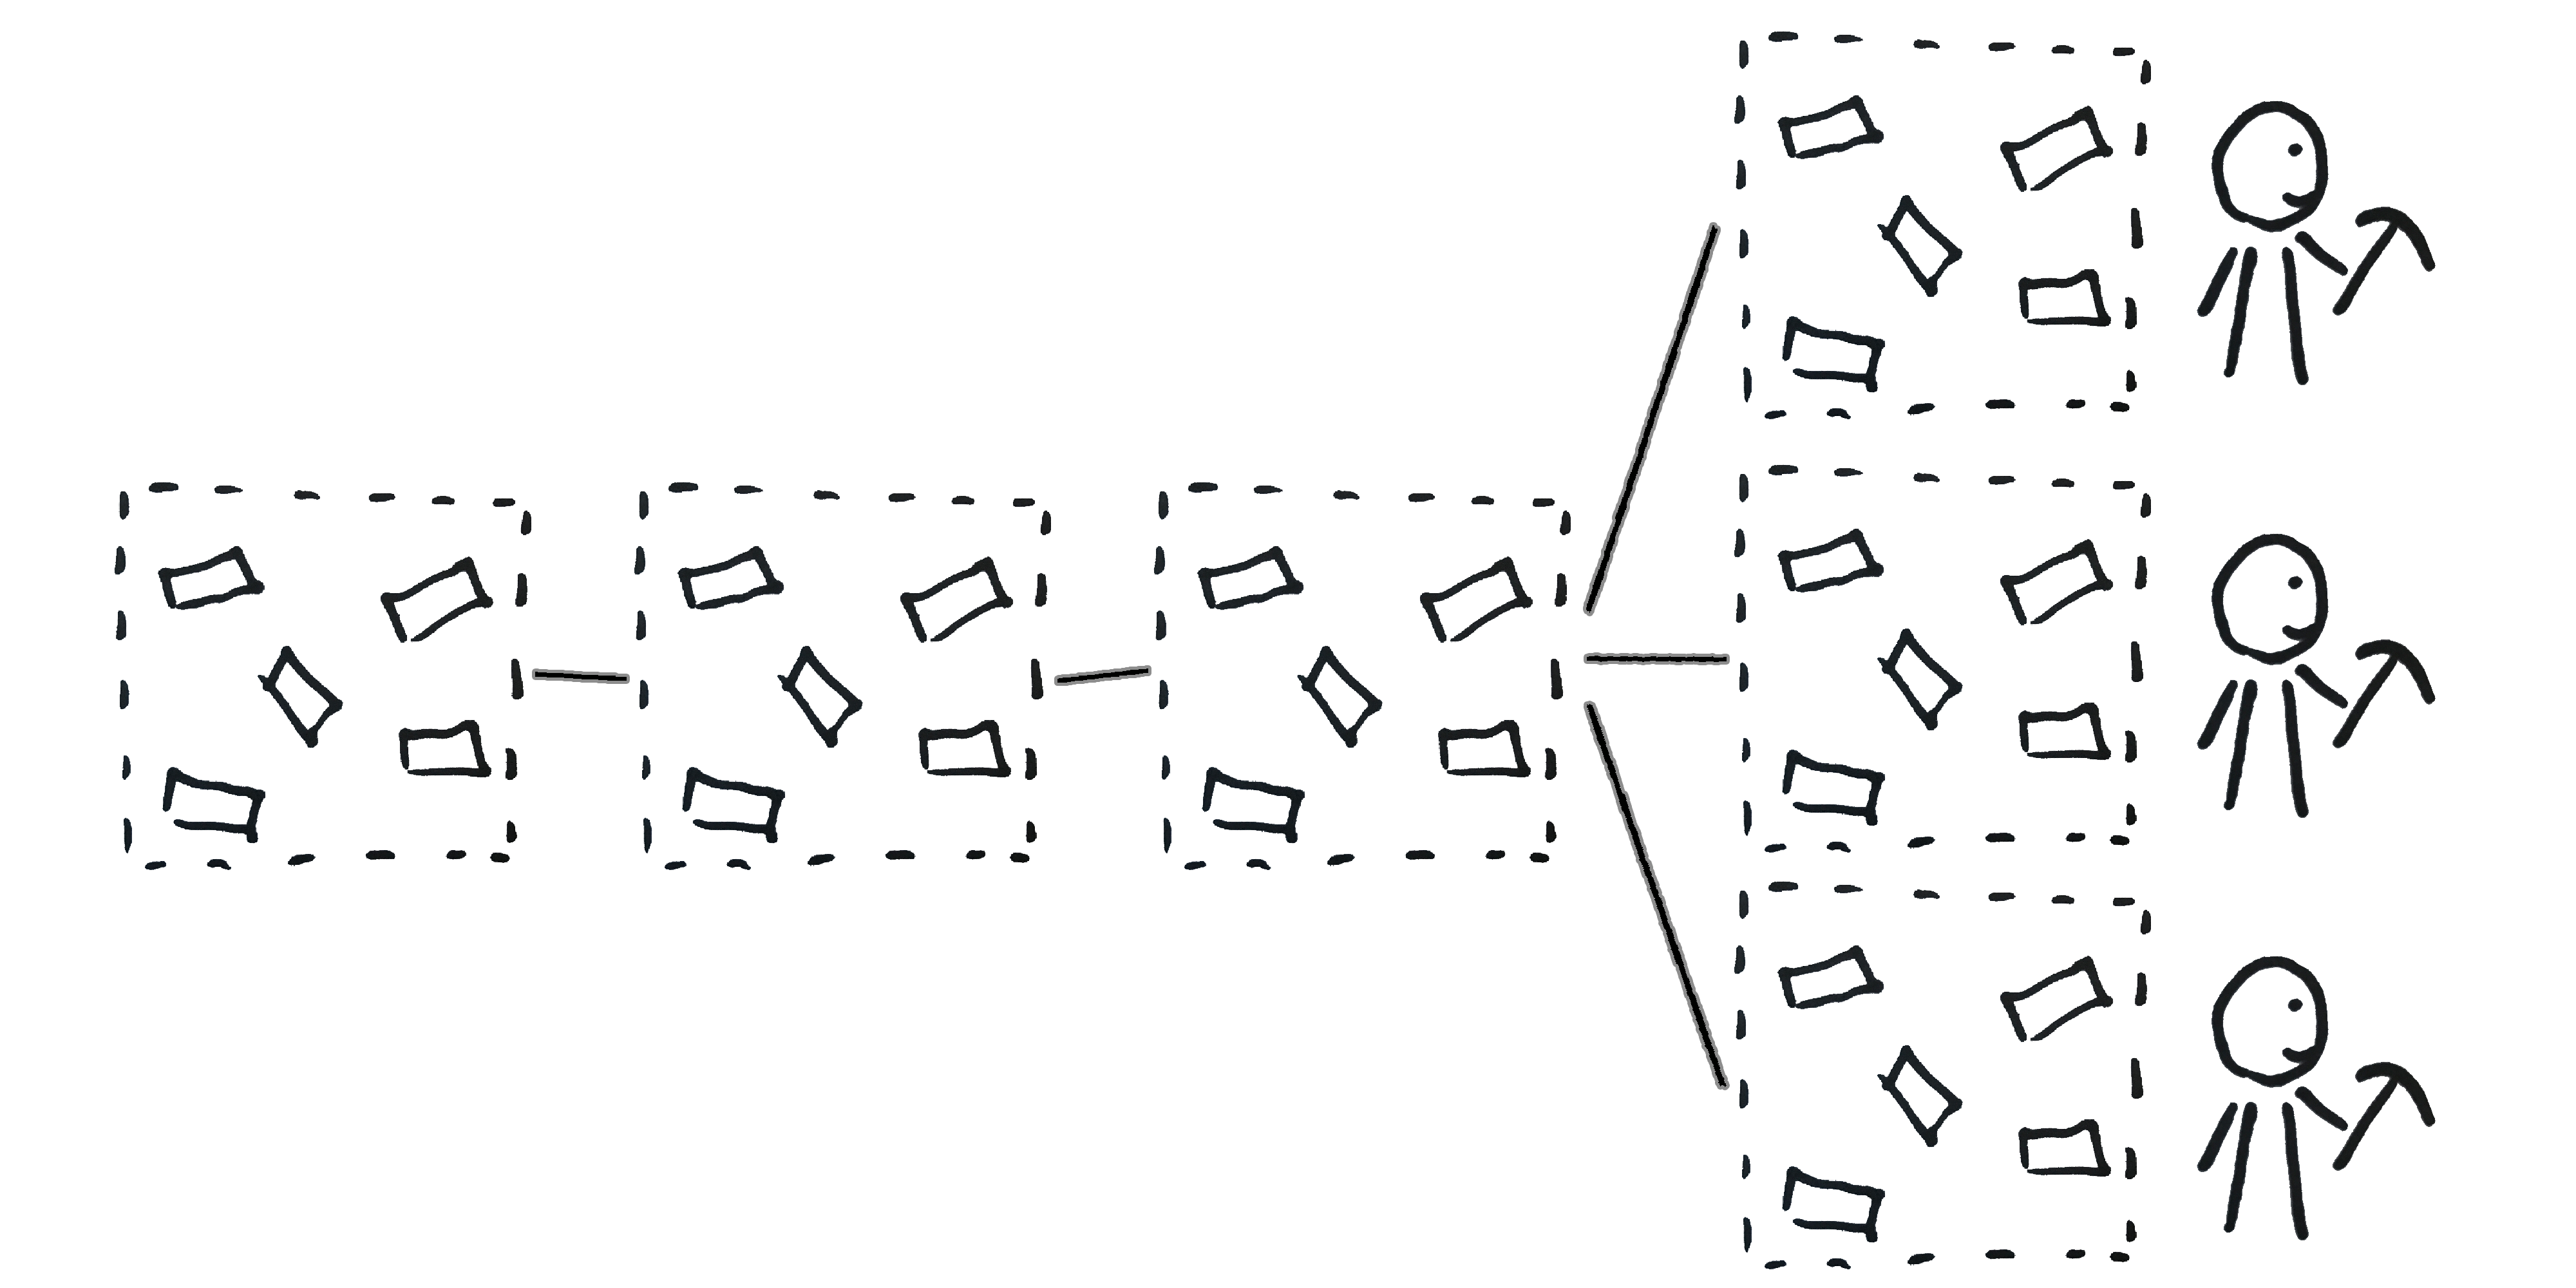
\includegraphics[width=9cm]{../assets/images/consensus_problem.png}

How to reach consensus?: \\
	\begin{itemize}
	\item Centralized decision (Proof-of-Authority)
	\item \color{focus}Decentralized lottery (Proof-of-Work)
	\end{itemize}
\end{frame}
%%%

%%%
\begin{frame}{Recommended Reading}
\begin{columns}
	\begin{column}{0.3\textwidth}
	\center
	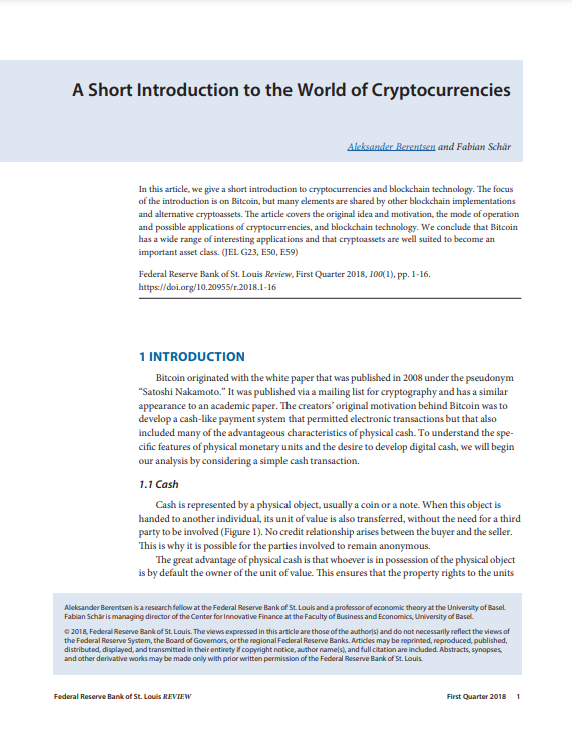
\includegraphics[width=\textwidth , frame]{../assets/images/short-introduction-cryptocurrencies.png}
	\end{column}
	\begin{column}{0.7\textwidth}
	\textbf{A Short Introduction to the World of Cryptocurrencies} \\
	Aleksander Berentsen and Fabian Schär \\
	\link \href{https://files.stlouisfed.org/files/htdocs/publications/review/2018/01/10/a-short-introduction-to-the-world-of-cryptocurrencies.pdf}{Online PDF}
	\end{column}
\end{columns}
\end{frame}

\end{document}
